% =======================
\documentclass[
  reprint,            % journal-like 2-column
  amsmath,amssymb,    % math packages
  aps,pre             % APS + Physical Review E style            
]{revtex4-2}

% ---- Core packages APS samples rely on ----
\usepackage{graphicx} % \includegraphics
\usepackage{dcolumn}  % decimal-aligned tables
\usepackage{bm}       % bold math
\usepackage[T1]{fontenc}
\usepackage[utf8]{inputenc}

% Hyperlinks (APS allows it; keep unobtrusive)
\usepackage[colorlinks=true, allcolors=blue]{hyperref}


% PACKAGES FOR LANGUAGE AND FONT
\usepackage{verbatim} % For code blocks

% PACKAGES FOR ALGORITHMS (PSEUDO-CODE)
\usepackage{etoolbox} 
\usepackage{algorithm}

% PACKAGES FOR IMAGES
\usepackage{tikz} % A package for high-quality hand-made figures.
\usetikzlibrary{}
\usepackage{float}
\usepackage[percent]{overpic} % For adding annotations to figures
\usepackage{graphbox} 

% FOR TABLES
\usepackage{array}     % enables m{...}, >{...}, \arraybackslash, etc.
\usepackage{booktabs}  % enables \toprule \midrule \bottomrule

% STANDARD MATH PACKAGES
\usepackage{mathtools}
\usepackage{cases}
\usepackage{xfrac}

% OTHER PACKAGES
\usepackage{lipsum} % DUMMY PACKAGE

% Graphics search paths (adjust as you like)
% You can keep just {Images/} and reference subfolders in filenames,
% or list subfolders explicitly as below.
\graphicspath{
  {Images/}
  {Images/Introduction/}
  {Images/Chapter 2/}
}

% Miscellaneous operators
\DeclareMathOperator{\arctanh}{arctanh}

\newcommand{\bea}{\begin{eqnarray}} % Shortcut for equation arrays
\newcommand{\eea}{\end{eqnarray}}
\newcommand{\e}[1]{\times 10^{#1}}  % Powers of 10 notation
\def\norm#1{\|#1\|} %Norm

% Commonly used symbols
\renewcommand{\a}{\alpha}
\renewcommand{\b}{\beta}
\renewcommand{\k}{\kappa}
\newcommand{\w}{\omega}
\newcommand{\wB}{\omega_B}
\newcommand{\wZ}{\omega_0}
\newcommand{\wz}{\omega_z}
\newcommand{\wpm}{\omega_\pm}
\newcommand{\neff}{n_{eff}}
\newcommand{\dn}{\delta n}
\newcommand{\dnbar}{\overline{\delta n}_{eff}}
\newcommand{\dt}{\delta \tau}

\newcommand{\Skenderas}{Sk\"{e}nderas}

\pdfpageattr{/Rotate 0}

% =======================
% Document
% =======================
\begin{document}

\preprint{APS/123-QED} % optional

\title{Modelling and Analysis of Semiconductor Lasers Under Fiber Bragg Grating Feedback}

% --- Example author block (edit to suit) ---
\author{First A. Author}
\affiliation{Your Department, Your University, City, Country}
\author{Second B. Author}
\email{second.author@example.edu}
\affiliation{Another Affiliation, City, Country}
\date{\today}

% ---- Abstract kept modular: put the whole environment in Sections/Abstract.tex ----

% !TeX root = ../main.tex

\begin{abstract}
Semiconductor lasers are compact, efficient light sources widely used in optical communications, and their sensitivity to external feedback makes them rich systems for studying nonlinear dynamics. The Lang-Kobayashi (LK) equations are the standard tool for modelling lasers subject to external feedback from a regular mirror. A key reflective component in optical systems is the fiber Bragg grating (FBG)—a periodic optical fiber refractive index variation—leveraged for its precise spectral control and all-fiber compatibility. When the external feedback comes from an FBG, present modelling requires a computationally expensive convolution term, which provides limited analytical insight into the system’s behaviour. We present a novel modelling approach that approximates FBG feedback by a sum of discrete delay terms. Critically, this avoids the need for numerical convolution while preserving the essential physics. This enables detailed analysis of the laser’s mode structure, stability regimes, and bifurcation structure in the spirit of that for the ‘classic’ LK equations. In this way, our work provides a foundation for deeper theoretical study of semiconductor lasers subject to technologically relevant types of FBG feedback, bridging the gap between numerical simulation and analytical understanding.
\end{abstract}


%\keywords{Suggested keywords}%Use showkeys class option if keyword
                              %display desired

\maketitle

% =======================
% Main text (modular)
% =======================
% Use \include so each section gets its own .aux (these will land in build/Sections/ with your latexmkrc)
% File names below are examples; create the matching files in Sections/ with no spaces in names.
% !TeX root = ../main.tex
\section{Introduction}
\label{sec:introduction}
%
Semiconductor lasers are crucial components in many technological applications. They have the advantage that their emission wavelengths are very popular as light sources in optical communication networks, while offering considerably smaller sizes (fractions of a millimetre) compared to the typical helium-neon lasers (tens of centimetres) allowing for their use across a plethora of practical applications \cite{vantartwijk1995semiconductor}. Semiconductor lasers are not only smaller than conventional lasers, but also significantly more open, allowing about 70\% of light intensity to escape, compared to the 1-5\% typical of conventional lasers. However, this openness makes semiconductor lasers more susceptible to external disturbances, resulting in a strong reaction to outside signals, which, albeit undesirable in practical applications, can be a promising route into the study of the potential nonlinear dynamics that can be produced with semiconductor lasers.
%
%
\section*{Lang Kobayashi equations}
\label{sec:LK}
%
The influence of external light on the operation of a laser has been studied in detail since the 1970s through the mechanisms of optical feedback (both conventional (COF) and phase-conjugate (POF)) and optical injection \cite{weiss1991dynamics}. The feedback and injection mechanisms have important practical implications; the former, for example, could be encountered in the operation of CD players, while the latter could be encountered in laser amplification systems. From a dynamical systems perspective, a significant breakthrough in the analysis of semiconductor laser dynamics came in 1980 through the seminal paper by Lang and Kobayashi, who introduced the so-called Lang Kobayashi (LK) rate equations describing the dynamics of a semiconductor laser under COF from a distant external mirror \cite{lang1980external}. A conceptual setup of this system is provided in Figure~\ref{fig:COF}. The LK equations describe the time evolution of the complex electric field $E = E_x + i E_y$ and the inversion (number of electron-hole pairs) $N$ inside the laser under the influence of external feedback $F(t) = \eta e^{-i\wZ\tau} E(t-\tau)$. A non-dimensionalised form of these equations that distils the key parameters governing the dynamics of this system is given by \eqref{eq:LK} \cite{heil2003delay}.
%
\begin{figure}[!t]
    \centering
    
    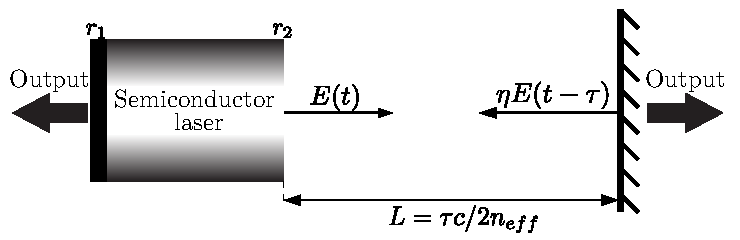
\includegraphics[width=0.7\linewidth]{Images/Introduction/COF_setup.pdf}
    
    \caption{Sketch of a semiconductor laser receiving feedback from an external mirror at distance $L$, leading to a delay time of $\tau=2L\neff/c$.}
    
    \label{fig:COF}
\end{figure}
%
\begin{equation}
\label{eq:LK}
    \begin{aligned}
        \frac{d E}{d t} & =(1+i \a) N(t) E(t)+\eta e^{-i C_p} E(t-\tau) \\
        T \frac{d N}{d t} & =P-N(t)-(1+2 N(t))|E(t)|^2
    \end{aligned}
\end{equation}
%
These key parameters can be separated into laser and external cavity (EC) parameters. The laser, which emits light at a single frequency $\w_0$ is characterised by the pump current $P$, the linewidth enhancement factor $\alpha$, and the ratio of photon and electron decay times $T = \tau_e/\tau_p$. The EC is characterised by the EC delay time $\tau = 2L\neff/c$, the feedback power level (ratio of power from the external mirror to that from the diode mirror) $\eta$, and the feedback phase $C_p = \w_0 \tau$, which is equal to the number of optical wavelengths in the EC. Treating the feedback phase as an independent parameter to the delay $\tau$ simplifies the analysis of the system while being physically justified for standard cavity lengths which are on the order of centimetres. Consider Figure~\ref{fig:Cp}, where the phase of the electric field in the EC is marked with white circles for two different EC lengths. The in length in the EC is less than the wavelength of the light, meaning that $L_{EC,1}\approx L_{EC,2}$. Therefore the change in the delay times between these cases is negligible. Comparing this to the large change in the phase - which shifts by $2\pi$ as the cavity length changes by half a wavelength due to the forward and backward propagation of the feedback signal within the cavity - to the negligible change in delay time, it is clear that on can treat the phase change $C_p$ as being independent from $\tau$. These equations are formulated with reference to the centre frequency of the laser, that is, we consider $\wZ = 0$ at the operating frequency, thus implying that $C_p=0$ in the first instance. Varying $C_p$ over a full $2\pi$ then amounts to changing the mirror position less than micron for wavelengths corresponding to visible light, using for example a piezoelectric transducer \cite{heil2003delay}. The application of these equations requires a single-mode laser system under the influence of weak feedback (up to a few \% of emitted light) from a long EC ($\mathcal{O}(\text{cm}) - \mathcal{O}(\text{m})$). Physically, the feedback rate $\eta$ is controlled by the reflectivities of the front facet $R_2$ and the external mirror $R$ and is given by the well-known expression 
%
\begin{figure}[!t]
    \centering
    
    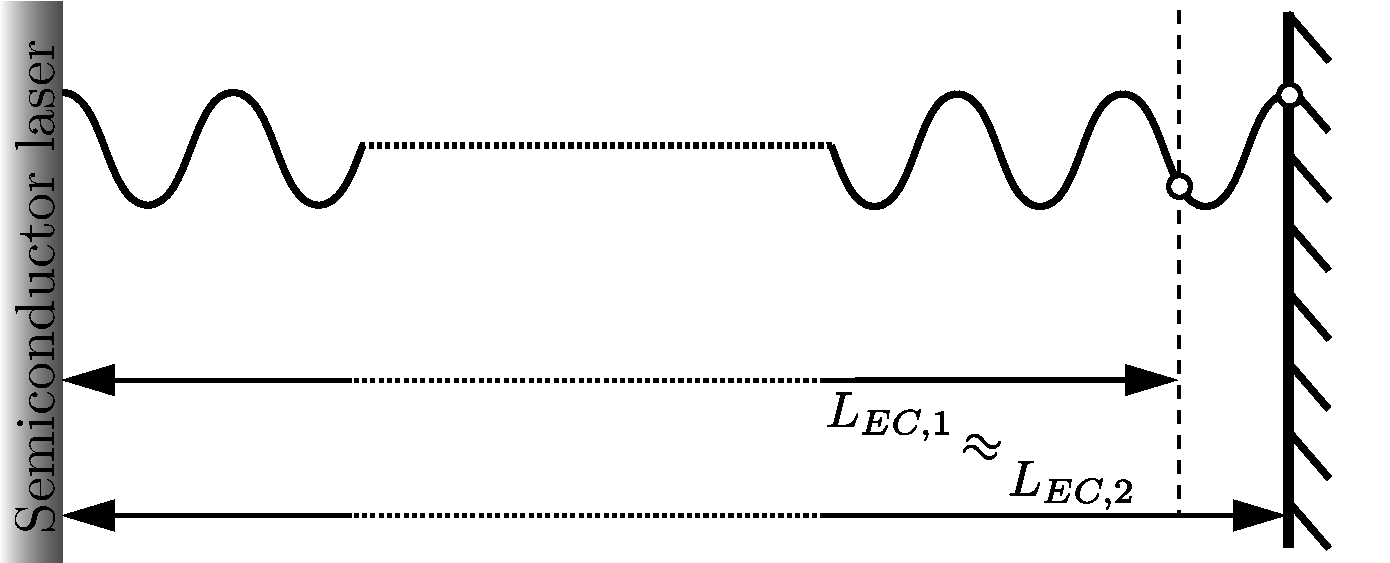
\includegraphics[width=0.65\linewidth]{Images/Introduction/Cp diagram.pdf}
    
    \caption{Illustration of the variation of phase in the EC for different lengths $L_{EC,1}$ and $L_{EC,2}$.}
    
    \label{fig:Cp}
\end{figure}
%
\begin{equation}
    \eta = \frac{(1-R_2^{\;2})R}{R_2}
\end{equation}
%
and is commonly kept low by using an anti-reflection coating for the front laser facet, ensuring $R_2$ and thus $\eta \ll 1$. Weak feedback ensures that multiple EC reflections between the front facet of the laser and the external mirror can be neglected. if this is not satisfied, the feedback $F(t)$ is more complex, taking the form \cite{vantartwijk1995semiconductor}
%
\begin{equation}
\label{eq:multiple_EC}
    F(t) = \frac{R_2^{\;2} - 1}{R_2^{\;2}} \sum_{n=1}^\infty (-R_2 R)^n e^{-i n C_p} E(t-n \tau)
\end{equation}
%
The LK equations have been shown to successfully describe a plethora of the complex dynamics observed in semiconductor lasers under weak external feedback, including steady-state, periodic, quasi-periodic, and chaotic emission, as well as more exotic behaviour such as regular pulse packages (RPPs), coherence collapse (CC), and low-frequency fluctuations (LFFs) \cite{heil1998coexistence}. The presence of the delayed feedback term $E(t-\tau)$ means that the LK equations are delay-differential equations (DDEs) whose phase space is the infinite-dimensional space $C[-\tau, 0]$ of continuous functions with values in $(E,N)$-space. It should be noted that this `memory' feature associated with optical feedback, where the system's evolution depends not only on its current state but also on past states due to time-delayed feedback, is not present when dealing with injected semiconductor laser systems.
%
\par
%
The LK equations' success can be attributed to the fact that their formulation as a system of coupled nonlinear DDEs is sufficient to give rise to rich dynamics observed in experiment, while simultaneously being amenable to mathematical analysis. The LK equations can be analysed in detail analytically, providing a deep understanding of the systems equilibria, creation/annihilation of steady state solutions through saddle-node (SN) bifurcations, and loss of stability through Hopf bifurcations \cite{rottschafer2007ecm}. In addition, with the advent of DDE numerical continuation software packages such as DDE-Biftool \cite{sieber2014dde}, the complex observed dynamics have been analysed and characterised in great detail \cite{krauskopf2004dynamics}.
%
\par
%
A key insight provided by the LK equations into the complex dynamics observed in semiconductor lasers under COF is the structure of steady-state solutions of the system, referred to as EC modes (ECMs). ECMs exist in the well known ellipse of ECMs centred at the lasers free-running frequency, with the most stable mode, referred to as the maximum gain mode (MGM) lying on the edge of the ellipse, that is, furthest from the centre frequency. The number of available ECMs and the frequency range they occupy depends on the feedback rate of the external mirror and generally increase with the feedback rate and cavity length. Trajectories of $(E,N)$ in phase space can `wrap around' the ECMs, these trajectories and thus the lasers dynamics increase in complexity for larger ellipses of ECMs \cite{heil2003delay}. A natural question that arose following this insight is the possibility of suppressing the number and bandwidth of available ECMs, increasing the lasers stability when exposed to larger amounts of external feedback.
%
%
\section*{Filtered optical feedback}
\label{sec:FOF}
%
The most natural method to suppress the frequency of emitted frequencies in a semiconductor laser is by filtering the externally fed back light, referred to as filtered optical feedback (FOF). Several practical implementations of this have been studied in the past. For example, the inclusion of a Fabry-P\'erot resonator within the feedback loop \cite{detienne1997semiconductor} and most notably, replacing the external mirror with a frequency selective surface, such as a grating \cite{dahmani1987frequency, harvey1991external, jin1996single}, or phase conjugating surface, for example, a Kerr-type nonlinear medium which has been shown to filter feedback \cite{agrawal1984line}. As expected in each of these cases, significant linewidth narrowing is observed leading to more stable operation around the filters free-running frequency. 
%
\begin{figure}
    \centering
    
    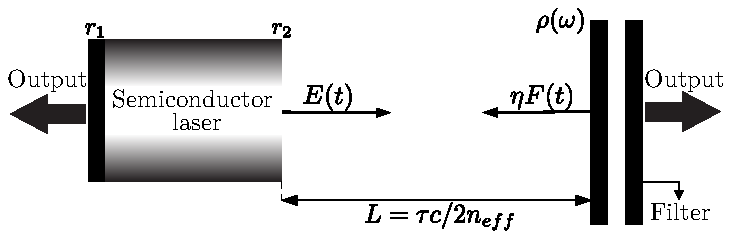
\includegraphics[width=0.7\linewidth]{Images/Introduction/FOF_setup.pdf}
    
    \caption{Sketch of a semiconductor laser receiving feedback from an external filtering mirror at distance $L$, leading to a delay time of $\tau=2 L \neff/c$.}
    
    \label{fig:FOF}
\end{figure}
%
\par
%
Mathematical analysis of FOF poses additional challenges. Now, the spectral components of the electric field must be accounted as their reflection is dictated by the frequency response of the chosen filter, defined as $\rho(\w)$. Therefore, the feedback term $\eta E(t-\tau)$ present in the LK equations must be replaced by a more complicated feedback term $\eta F(t)$ to account for this frequency selectivity. For a particular reflection response, the term $F(t)$ can be calculated by decomposing the field into its Fourier components, letting the filters reflectivity spectrum $\rho(\w)$ operate on it, and finally taking the inverse Fourier transform \cite{yousefi1999dynamical}.
%
\begin{equation}
    \begin{aligned}
    \label{eq:FOF}
         F(t) &=  \mathcal{F}^{-1}\big[ \mathcal{F}[E(t)](\w) \times \rho(\w) \big](t-\tau)\\
              &= \frac{1}{2\pi} \int_{-\infty}^{\infty} \rho(\w) \int_{-\infty}^{\infty} E(t') e^{-i \w t'} dt' e^{i \w (t-\tau)} d\w
    \end{aligned}
\end{equation}
%
Note that \eqref{eq:FOF} again assumes a single reflection to be sufficient to describe the external feedback signal $\eta F(t)$. This expression for the distributed external feedback is generally challenging to analyse both analytically and numerically. The modified LK equations are now integro-differential equations which are not amenable to standard tools of bifurcation analysis such as the calculation of fixed points and their stability, clouding even basic insights into the influence of filtering on the system. Further, numerical methods such as the integration of time series for $(E,N)$ are significantly more computationally expensive, as now \eqref{eq:FOF} must be calculated at each time step, rather than simply using the stored value $E(t-\tau)$ as in the case of the standard LK equations.
%
\par
%
A key insight was made in 1999 by Yousefi and Lenstra \cite{yousefi1999dynamical} by assuming that filtering leads to a frequency-dependent reflectivity spectrum $\rho(\w)$ composed of a sum of Lorentzians. By considering a single Lorentzian (and $A_0=1$), which may be sufficient to describe certain external feedback mechanisms \cite{dahmani1987frequency,detienne1997semiconductor}, they showed that integro-differential equations for the distributed FOF can be converted to a system of DDEs.
%
\begin{equation}
    \begin{aligned}
    \label{eq:FOF_LK}
        \frac{d E}{d t} &= (1+i \alpha) N(t) E(t)+\eta F(t) \\
        T \frac{d N}{d t} &= P - N(t) - (1 + 2 N(t))|E(t)|^2 \\
        \frac{d F}{d t} &= \lambda E(t-\tau) e^{-i C_p}+(i \Delta-\lambda) F(t)
    \end{aligned}
\end{equation}
%
where $\Lambda$ is the full width half maximum (FWHM) of the filter, thus controlling the filter's spectral width, and $\Delta$ is the detuning of the Lorentzian filter from the laser's free-running frequency. As \eqref{eq:FOF_LK} are simply a system of DDEs, they are amenable to all analytical methods and numerical methods available to the original LK equations. They demonstrated that as expected, the system generally has fewer ECMs available compared to COF and that, globally speaking, the filtering leads to more stable dynamics. Alongside the reduction of the available ECMs, the MGM tends to lie nearer to the filter frequency (but not precisely at it) rather than at the edge of the fixed point ellipse as in the case of COF. The form of these equations as coupled DDEs allows for detailed analysis through continuation and stability analysis of these stationary states, providing deep insights into the influence of FOF on semiconductor lasers \cite{erzgraber2006frequency, erzgraber2007bifurcation, erzgraber2007dynamics, fischer2000experimental, fischer2004experimental, green2006mode, hek2007semiconductor, erzgraber2007feedback, fischer2004filtered, yousefi2001global, yousefi2002simulations, yousefi2003nonlinear}. 
%
%
\section*{Fiber Bragg gratings}
\label{sec:FBG}
%
One such frequency selective component which has been the subject of extensive research in recent decades are fiber Bragg gratings (FBGs). FBGs have several advantages over other fiber optic technologies. They offer all-fiber design, low insertion loss, high return loss or extinction,  potential for lower costs, and most notably, exceptional flexibility in achieving specific spectral characteristics. With current manufacturing techniques, it is possible to create gratings with near arbitrary spectral responses $\rho_\text{Bragg}(\w)$ and normalized bandwidths ranging from $0.1$ to $10^{-4}$ \cite{erdogan1997fiber}. The FBG is therefore a natural reflective component to enable FOF.
%
\begin{figure}
    \centering
    
    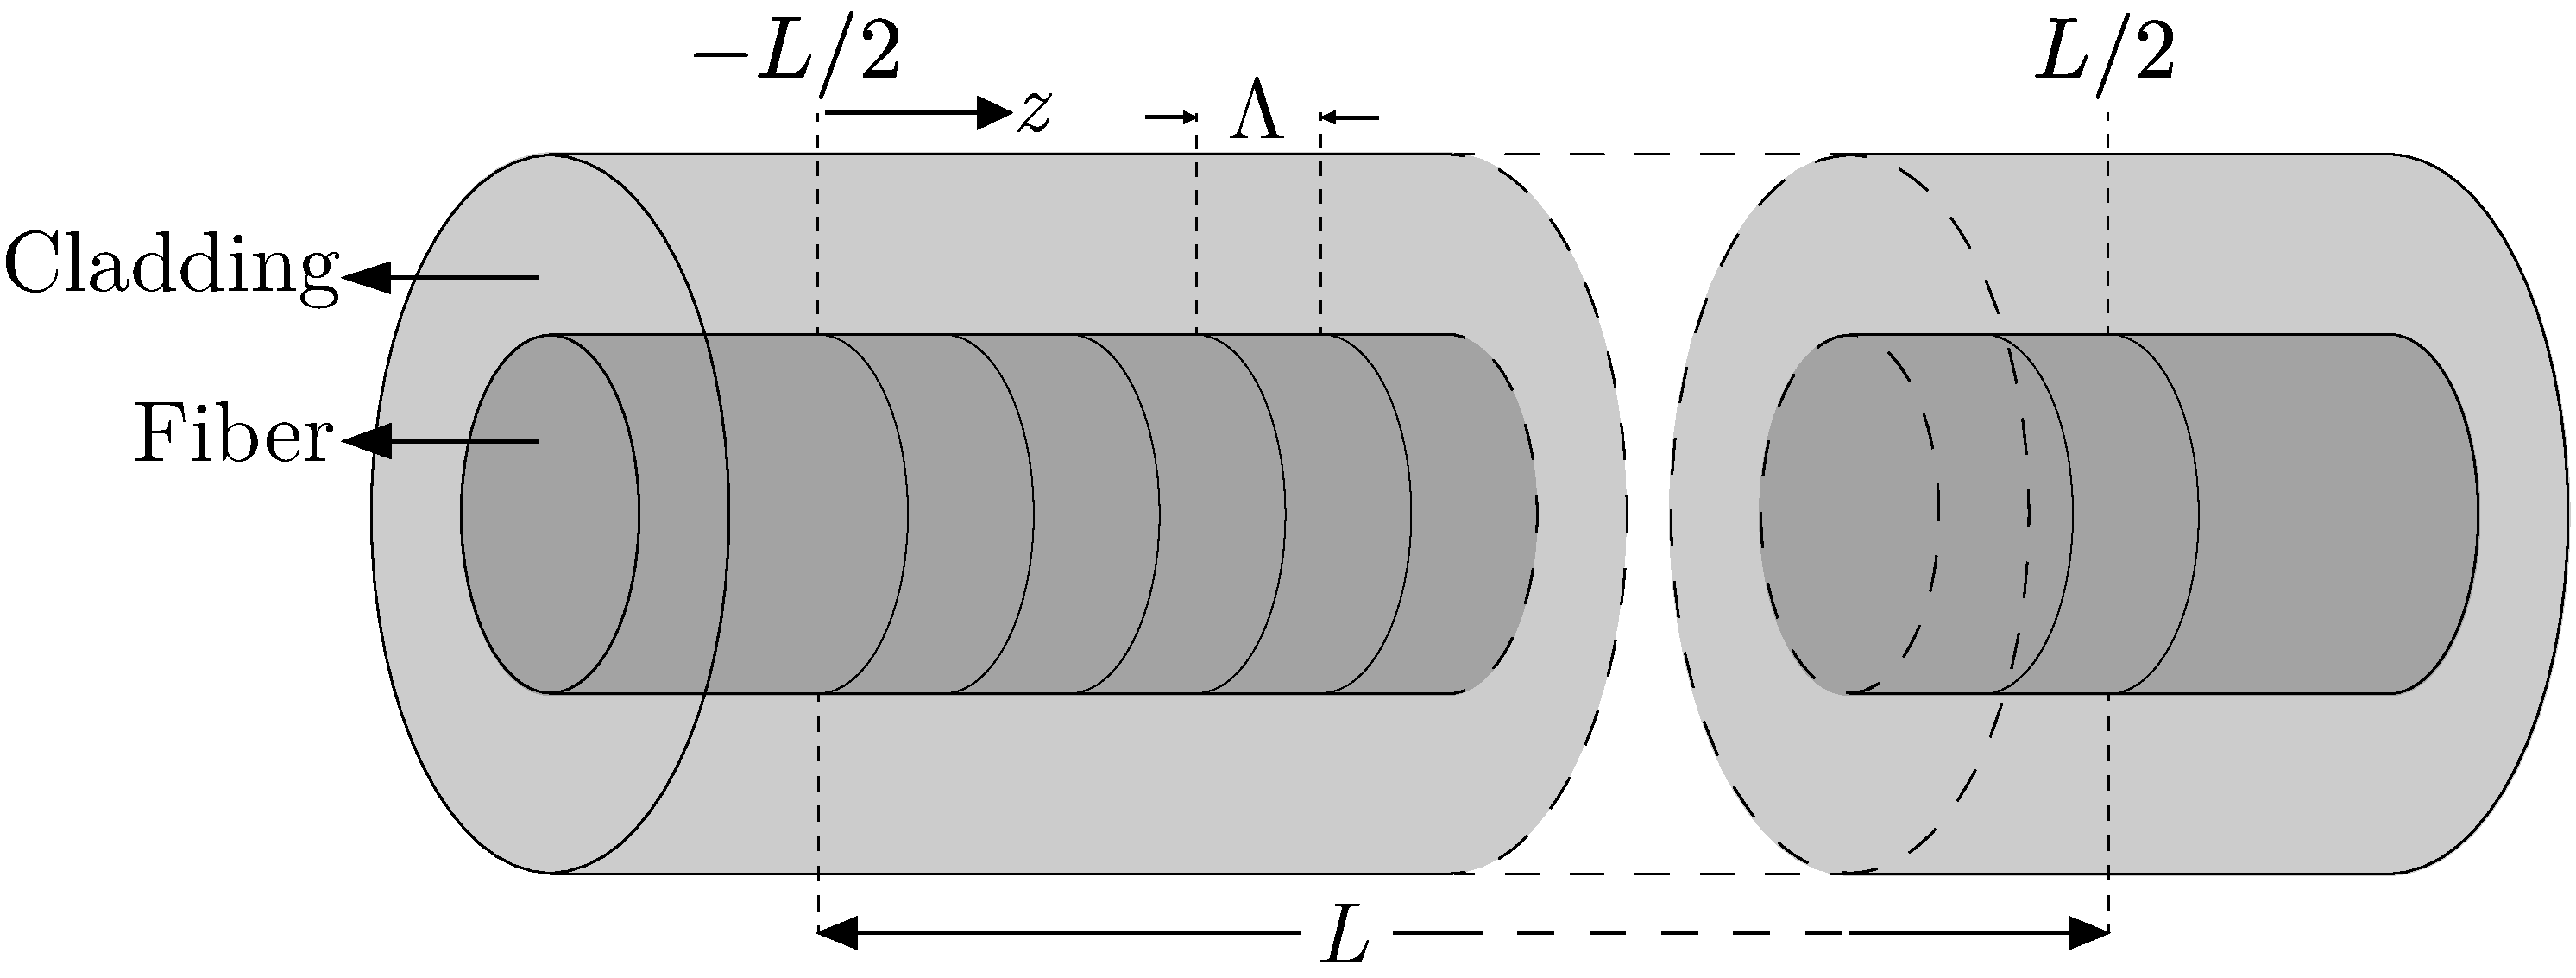
\includegraphics[width=0.7\linewidth]{Images/Introduction/FBG.pdf}
    
    \caption{Sketch of an optical fiber with an FBG written along its length.}
    
    \label{fig:FBG}
\end{figure}
%
\par
%
A sketch of an FBG written into an optical fiber is shown in Figure~\ref{fig:FBG}. It is defined as a repeating periodic variation $\delta n_{eff}(z)$ of the refractive index every $\Lambda$ along a length $L$ of a fiber. The number of gratings along an FBG is therefore $N = L/\Lambda$. The most general form for this periodic variation is given by
%
\begin{equation}
\label{eq:dneff}
    \delta n_{eff}(z) = \dnbar(z) \left[ 1 + v \cos{\left( \frac{2 \pi}{\Lambda} z + \phi(z) \right)} \right]
\end{equation}
%
where $\Lambda$ is the period of the grating, $\dnbar(z)$ is the profile of the periodic variations over $L$, for example, $\dnbar(z) \sim e^{-z^2}$ produces a Gaussian variation to the profile of the refractive index variation, $v$ is the fringe visibility of the index change, and $\phi(z)$ can vary the grating period along the fiber, allowing different frequencies to be reflected along the fiber's length.
%
\begin{figure}[!t]
    \centering
    \begin{overpic}[width=0.4\linewidth]{Images/Introduction/Uniform grating.pdf}
        \put(3,65){(a)}
    \end{overpic}
    \begin{overpic}[width=0.4\linewidth]{Images/Introduction/Gaussian apodized grating.pdf}
        \put(3,65){(b)}
    \end{overpic}
    \\
    \begin{overpic}[width=0.4\linewidth]{Images/Introduction/Chirped grating.pdf}
        \put(3,65){(c)}
    \end{overpic}
    \begin{overpic}[width=0.4\linewidth]{Images/Introduction/Phase shift grating.pdf} 
        \put(3,65){(d)}
    \end{overpic}
    
    \caption{Some examples of common types of FBGs as classified by variation of $\delta n_{eff}(z)$, including (a) uniform with positive-only index change, (b) Gaussian-apodized, (c) chirped, and discrete phase shift.}
    
    \label{fig:dneff}
\end{figure}
%
\par
%
Light propagating through the fiber that interfaces with the FBG can undergo diffraction when its wavelength close to the design wavelength, given by $\lambda_D = 2 \neff \Lambda$. It is typically assumed that the light only undergoes first-order diffraction as this typically dominates in FBGs and thus a single propagating mode is considered. In this case, through the use of coupled-mode theory and the synchronous approximation, coupled first-order differential equations describing the interaction between the forward and backward propagating waves, $A(z)$ and $B(z)$, respectively, can be derived. See \cite{erdogan1997fiber} and references therein for further details.
%
\begin{equation}
\label{eq:wave_eqs}
    \begin{aligned}
        \frac{dR}{dz} &= i \hat{\sigma} R(z) + i \k S(z), \, R(z) = A(z) \exp{ \left( -i \left( \frac{\phi}{2} -\delta z \right) \right) }\\
        -\frac{dS}{dz} &= i \hat{\sigma} S(z) + i \k R(z), \, S(z) = B(z) \exp{ \left( -i \left( \frac{\phi}{2} + \delta z \right) \right) }
    \end{aligned}
\end{equation}
%
The terms $\delta$, referred to as the detuning, $\k$, referred to as the "AC" coupling coefficient and $\hat{\sigma}$, referred to as the general "dc" self-coupling coefficient, are given by
%
\begin{align}
    \label{eq:delta}
    \delta &= 2 \pi \neff \left( \frac{1}{\lambda} - \frac{1}{\lambda_D} \right) \\
    \label{eq:kappa}
    \k &= \frac{\pi}{\lambda} v \dnbar(z)\\
    \label{eq:sigma}
    \hat{\sigma} &= \frac{2\k}{v} + \delta -\frac{1}{2}\frac{d\phi}{dz}
\end{align}
%
As $\k$ and $\hat{\sigma}$ generally depend on $z$, \eqref{eq:wave_eqs} cannot usually be solved analytically, but they are easily solved numerically following the prescription of a particular $\Lambda$, $\neff$, $\dnbar(z)$, $\phi(z)$, and $L$. 
%
\par
%
At this point, we have all the necessary ingredients to calculate the key characteristic of an FBG - its reflectivity spectrum $\rho(\w)$. Physically speaking, one is most interested in the reflection spectrum of light being reflected at the front FBG interface with no reflection at the back FBG interface. Therefore, \eqref{eq:wave_eqs} is typically solved (by defining $z=0$ to be half way along the FBGs length) subject to the boundary conditions $R(-L/2)=1$ and $S(L/2)=0$ and integrating backwards from $L/2$ to $-L/2$, with the amplitude reflection coefficient then given by
%
\begin{equation}
\label{eq:rho}
    \rho = \frac{S(-L/2)}{R(-L/2)}
\end{equation}
%
Although closed-form expressions for $\rho(\w)$ are typically not possible, as \eqref{eq:wave_eqs} must be solved numerically, some commonly used gratings allow for analytic expressions for $\rho(\w)$ and thus give excellent insights into common properties of FBG reflection spectra.
%
%
\subsection*{Uniform FBG reflection spectra $\rho_\text{Bragg}(\w)$}
\label{subsec:FBG_feedback}
%
The most basic FBG is called the uniform grating. Its grating chirp $\sfrac{d\phi}{dz} = 0$ and the apodization $\dnbar=\text{const.}$ so that its grating index variation given by $\eqref{eq:dneff}$ is essentially a sine wave as shown in Figure~\ref{fig:dneff}(a). Therefore, $\k, \, \hat{\sigma}$ are constant in $z$, allowing an analytic reflectivity spectrum $\rho(\w)$ to be calculated by solving \eqref{eq:wave_eqs} and subsequently evaluating \eqref{eq:rho}.
%
\begin{equation}
\label{eq:uniform_rho}
    \rho = \frac{-\k \sinh\left(\sqrt{\k^2 - \hat{\sigma}^2}L\right)}{\hat{\sigma} \sinh\left(\sqrt{\k^2 - \hat{\sigma}^2}L\right) + i\sqrt{\k^2 - \hat{\sigma}^2} \cosh\left(\sqrt{\k^2 - \hat{\sigma}^2}L\right)}
\end{equation}
%
Several interesting features of reflection spectra $\rho$ are most easily visualised by varying $\k L$ for a particular fixed $N$ against normalised frequency, given by \cite{erdogan1997fiber}
%
\begin{equation*}
    \frac{\omega}{\omega_\text{max}} = 1 + \frac{\hat{\sigma} L}{\pi N}
\end{equation*}
%
Figure~\ref{fig:uniform_spectra_varykL} illustrates representative amplitude reflectivity and phase curves for uniform gratings plotted against angular frequency, for gratings centred at the most commonly used laser wavelength of 1550 nm, with values of $\k L \in [0.5, 2, 5]$, and a fixed $N = 5000$. Increasing $N$ (and therefore increasing $L$) results in a narrower reflection bandwidth, while decreasing $N$ (and therefore decreasing $L$) leads to a broader one, assuming $\k L$ remains constant. Reflection spectra consist of a main lobe and a series of side lobes, partitioned by reflection zeros, spaced symmetrically (as a function of $\lambda$) on either side of it. For gratings with a low $\k L$ such as 0.5, the main lobe was a bandwidth, which we define as the interval between its reflection zeros, equal to twice that of its side lobes \cite{erdogan1997fiber}. Evidently, increasing $\k L$ not only increases the grating's maximum reflectivity, but additionally broadens the bandwidth of the main lobe while narrowing the bandwidth of the side lobes. Additionally, the phase variations are approximately linear for low reflectivities while becoming more distorted as $\k L$ increases.
%
\begin{figure}
    \centering
    
    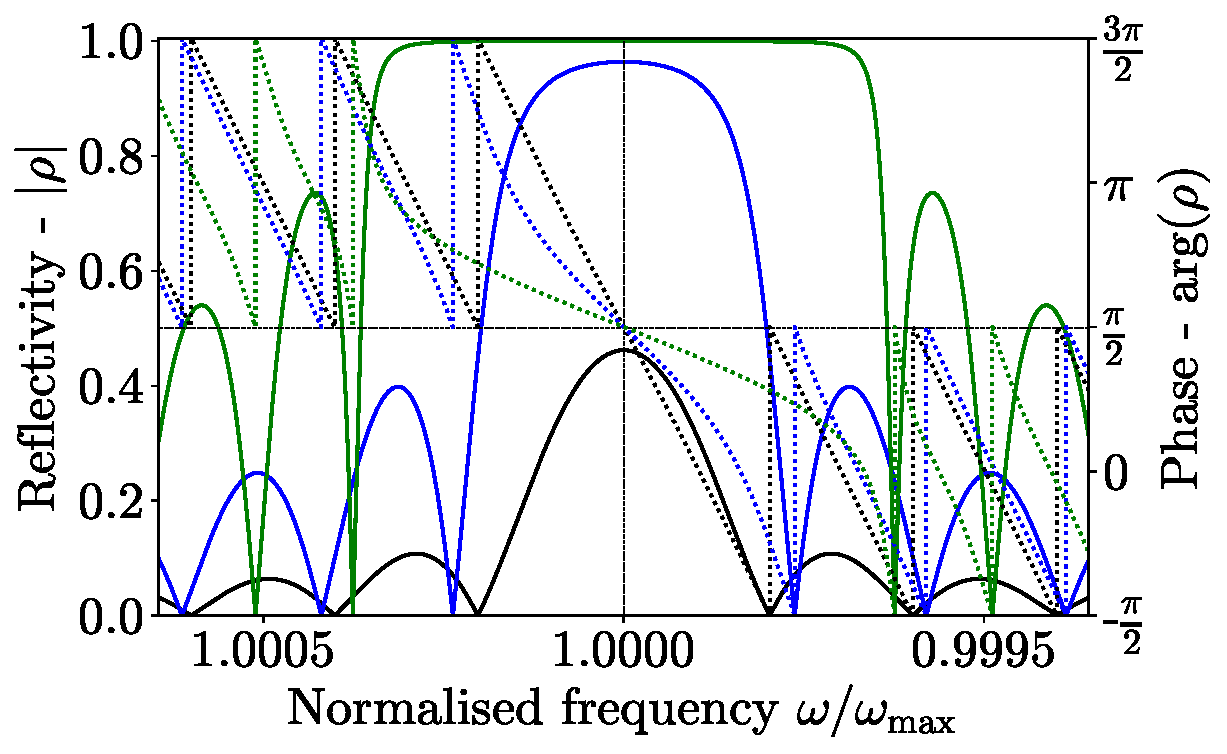
\includegraphics[width=0.6\linewidth]{Images/Introduction/Uniform varying kL.pdf}
    
    \caption{Examples of magnitude and phase of uniform FBG reflection spectra with varying $\k L \in [0.5, 2, 5]$ and constant $N=5000$.}
    
    \label{fig:uniform_spectra_varykL}
\end{figure}
%
\begin{figure}
    \centering
    
    \begin{overpic}[width=0.45\linewidth]{Images/Introduction/Uniform p constant dneff.pdf}
        \put(0,72){(a)}
    \end{overpic}
    \hspace{0.02\linewidth}
    \begin{overpic}[width=0.45\linewidth]{Images/Introduction/Uniform p constant L.pdf}
        \put(0,72){(b)}
    \end{overpic}
    
    \caption{Examples of magnitude and phase of uniform FBG reflection spectra demonstrating the effect of varying $\dnbar$ and $L$. The nominal case (black curves) in (a) and (b) are $\dnbar = 1\e{-2}\neff$ versus $L = 5\text{cm}$. In (a), the grating length is doubled to $L = 10\text{cm}$ (green curves) and in (b), the index change is doubled to $\dnbar = 4\e{-6}\neff$ (blue curves).}
    
    \label{fig:uniform_spectra_varyLdneff}
\end{figure}
%
\par
%
As $\k, \hat{\sigma}$ depend solely on $\lambda$ and the prescribed grating parameters, the reflected amplitude $|\rho|$ and reflected phase $\arg(\rho)$ can be immediately plotted against frequency by substituting \eqref{eq:kappa} and \eqref{eq:sigma} into \eqref{eq:uniform_rho}. Figure~\ref{fig:uniform_spectra_varyLdneff} shows some examples of the reflection spectra of uniform FBGs, now plotted against frequency, with their design frequency given by
%
\begin{equation}
    \w_D = \frac{\pi c}{\Lambda n_{eff}^2}
\end{equation}
%
highlighted to demonstrate the intrinsic detuning in the spectrum. The reflection spectrum of a uniform grating has a maximum reflectivity 
%
\begin{equation}
\label{eq:rmax}
    R \equiv |\rho_\text{max}| = \tanh{(\k L)}
\end{equation}
%
centred at the Bragg centre frequency $\w_c \equiv \omega_\text{max}$
%
\begin{equation}
\label{eq:wBragg}
    \w_c = \frac{\w_D}{\left( 1 + \frac{\dnbar }{\neff}\right)}
\end{equation}
%
We note that typically, $R$ is used for reflected power rather than reflected amplitude, but this choice of notation is made for clarity reasons in later sections. The phase at $\w_c$ is $\sfrac{\pi}{2}$ for all uniform gratings, while the reflection zeros are symmetric about $\w_c$, with the zeros either side of the main lobe occurring at $\w_c \pm \wz$, where
%
\begin{equation}
\label{eq:wz}
    \wz = \w_c \sqrt{\left( \frac{\dnbar}{2 \neff} \right)^2 + \frac{1}{N^2} }
\end{equation}
%
and the phase of the reflection spectrum varies by $2 \pi$ between the zeros. Outside of the main lobe, side lobe reflectivity peaks decay exponentially with periodic phase variations of $\pi$ within each lobe. Note the phase shift of $\pi$ between side lobes on either side of the reflectivity spectrum.
%
\par
%
Figure~\ref{fig:uniform_spectra_varyLdneff}(a) demonstrates the effect of doubling $L$ on reflection spectrum. Intuitively, $R$ increases for longer gratings as more gratings are available to prevent signal transmission. The bandwidth of each lobe decreases while the detuning from the design frequency is unchanged. When doubling $\dnbar$ as demonstrated in (b), $R$ is again increased. Conversely to (a), detuning increases while the grating bandwidth is unchanged. As these two parameters control the three features of the spectrum (detuning, maximum reflection, and bandwidth), one cannot vary a single feature of the reflection spectrum without additionally adjusting the grating period $\Lambda$, which can be used to compensate the detuning in $\w_c$ while having a negligible affect on $\wz$ and $R$. This is because optical lasers' centre frequencies are in THz while the amount of detuning is at most in GHz. Therefore, $\w_c/\w_D = \Lambda_D/\Lambda_c \approx 1$. Using this approximation, \eqref{eq:wBragg}, and \eqref{eq:wz}, $\dnbar, L, \Lambda$ can be calculated sequentially through the expressions
%
\begin{figure}
    \centering
    
    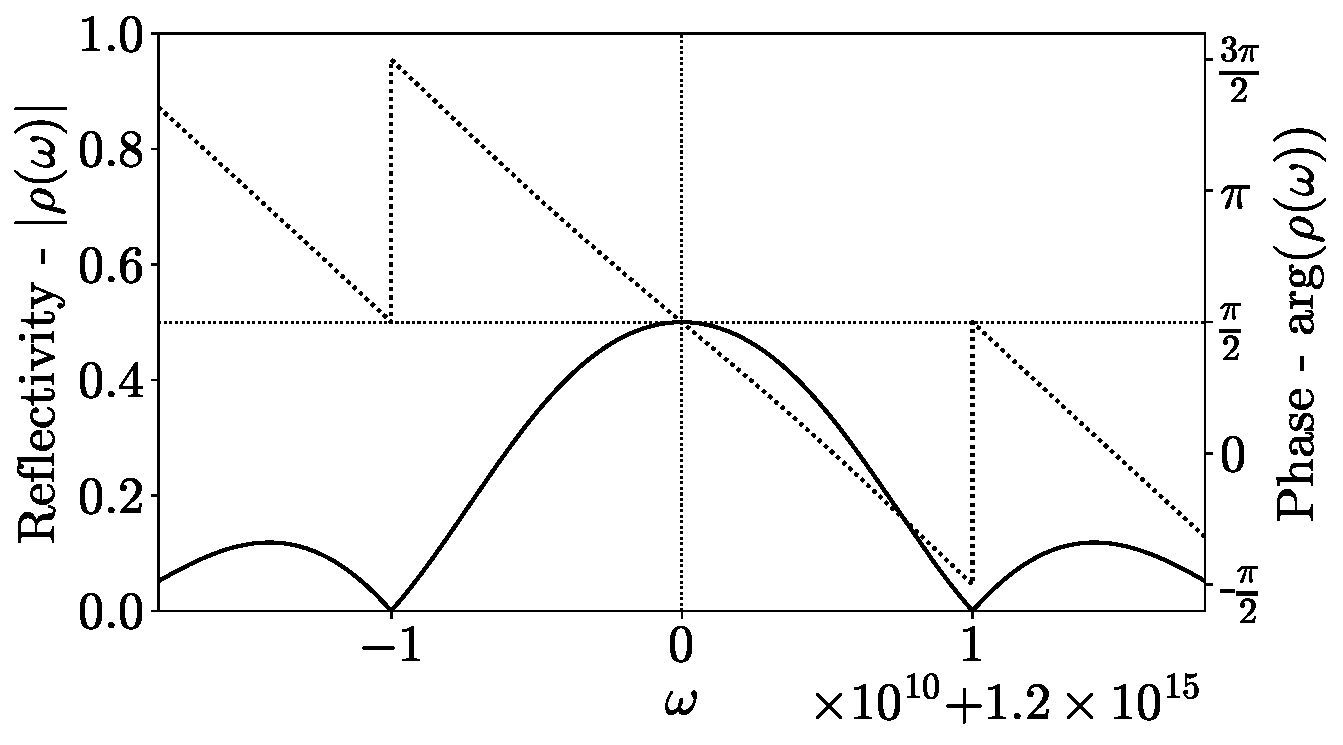
\includegraphics[width=0.65\linewidth]{Images/Introduction/spec2phys.pdf}
    
    \caption{Spectral response of a uniform grating with desired shape parameters $\w_c = 1.216\times 10^{15}$, $\wz = 10\e{10}$, and $R = 0.5$ using physical parameters $\dnbar= 4.2111838\e{-6}$, $\Lambda = 3.6494583\e{-7}\,\text{m}$, $L = 0.0444578955\,\text{m}$  calculated through \eqref{eq:spec2phys}.}
    
    \label{fig:spec2phys}
\end{figure}
%
\begin{align}
\label{eq:spec2phys}
    \dnbar &\approx \frac{2\wz}{\w_c} \frac{\neff}{\sqrt{1 + \left(\frac{\pi}{\arctanh{(R)}} \right)^2}}
    \\
    \Lambda &= \frac{\pi c}{\w_c \neff (\neff +\dnbar)}
    \\
    L &= \frac{\Lambda}{\sqrt{\left( \frac{\wz}{\w_c} \right)^2 - \left( \frac{\dnbar}{2\neff} \right)^2}}
\end{align}
%
For example, if a uniform grating with a spectral response corresponding to $\w_c = 1.216\e{15}\; \text{rad s}^{-1}$, $\wz = 1\e{10}\; \text{rad s}^{-1}$, and $R = 0.5$ is desired, \eqref{eq:spec2phys} provides grating parameters $\dnbar= 4.2111838\e{-6}$, $\Lambda = 3.6494583\e{-7}\,\text{m}$, $L = 0.0444578955\,\text{m}$, which gives excellent agreement to the desired spectral response as shown in Figure~\ref{fig:spec2phys}. 
%
%
\section*{FBG distributed feedback}
\label{sec:FBG_feedback}
%
Given the significant spectral advantages of FBGs for FOF and the straight-forward integration of FBGs into fiber optic semiconductor laser systems, investigations into their influence on the dynamics of external feedback semiconductor laser systems is of great interest. A sketch of the laser system under external feedback from an FBG is shown in Figure~\ref{fig:FBGF}. As demonstrated in the previous section, the reflectivity spectrum of FBGs can be rather complex. As an FBG in essence acts as a filter, the term $F(t)$ will be given by \eqref{eq:FOF} with $\rho(\w) = \rho_\text{Bragg}(\w)$. This term can alternatively be written as a convolution in the time domain,
%
\begin{equation}
    \label{eq:convolution}
     F(t) = e^{-i C_p} \tilde{\rho}_\text{Bragg}(t) \otimes E(t-\tau)
\end{equation}
%
where $\tilde{\rho}_\text{Bragg}(t)$ is the impulse response of the FBG with respect to the Bragg resonance frequency. Analytic expressions do not exist for the impulse response, even for simple gratings, and must therefore be calculated numerically through fast Fourier transforms (FFTs), for example. The requirement of numerically calculating $F(t)$ limits the analysis to numerical integration of solutions for $(E(t),N(t))$, and calculating properties of resulting time series, such as maximal Lyapunov exponents (MLEs) or spectral characteristics such as signal dispersion. Despite the obvious computational and analytical difficulties associated with this feedback term, research has been conducted into uniform FBG feedback using the convolution representation for $F(t)$ \cite{li2012distributed, li2015chaotic, li2020stable, jiang2021characterizing, skenderas2021feedback, skenderas2024impact}. In several studies, an expression for $\rho(\w)$ separates the reflection spectrum and detuning, allowing the detuning to be varied continuously while keeping the reflectivity spectrum shape constant. In this case, the reflected signal has the form,
%
\begin{equation*}
    F(t) = \eta e^{-i C_p} [\tilde{\rho}_0(t) e^{i \wB t}] \otimes E(t-\tau)
\end{equation*}
%
where $\tilde{\rho}_0$ is centred at the laser free-running frequency, while the detuning $\wB$ is an independent parameter. Although this form for the reflectivity distribution allows one to vary a single feature of the reflectivity distribution, as discussed in \ref{subsec:FBG_feedback}, the detuning and distribution shape intrinsically depend on each other, meaning that all grating parameters $\dnbar, \Lambda, L$ must be simultaneously adjusted in order to continuously detune over a constant distribution shape \cite{skenderas2024impact}. These parameters can be calculated for example through \eqref{eq:spec2phys}. Similarly, the distribution width and maximum reflectivity (occurring at $\w_c$) can only be independently varied through simultaneously varying all grating parameters.
%
\begin{figure}[!t]
    \centering
    
    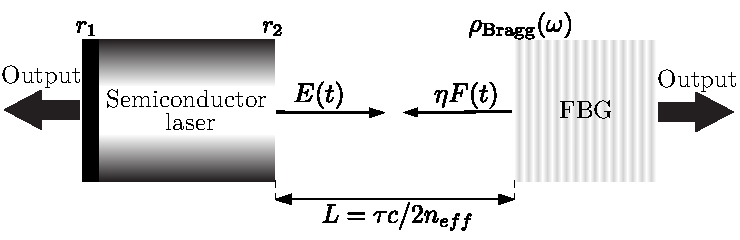
\includegraphics[width=0.7\linewidth]{Images/Introduction/FBG_setup.pdf}
    
    \caption{Sketch of a semiconductor laser receiving feedback from an external FBG at distance $L$, leading to a delay time of $\tau=2L\neff/c$.}
    
    \label{fig:FBGF}
\end{figure}
%
\par
%
As numerical investigations only allow limited insights into the underlying dynamics of FBG feedback, initial numerical investigations focused on the potential of FBG feedback to produce high-quality chaotic signals. This is of research interest as chaotic signals produced by lasers subject to external feedback are used in a number of applications such as high-speed optical random bit generation \cite{uchida2008fast} and chaos-based secure communication \cite{annovazzi2008secure}. It was demonstrated that FBG feedback is more effective than conventional mirror feedback in suppressing the time-delay signature (TDS) associated with chaos generation in semiconductor lasers. TDS can limit the encryption capabilities of chaotic signals generated lasers subject to external feedback, as powerful autocorrelation algorithms can use a signal's TDS to partially or fully decrypt the signal \cite{rontani2007loss}. The improvement in TDS suppression was generally attributed to the time-distributed reflections provided by the FBG, `spreading out' the effective time delay of the chaotic signal \cite{li2012distributed}. Further, it was observed that TDS suppression improves as the bandwidth of the FBG decreases. This is linked to the increase in dispersion of the reflection group delay, which plays a crucial role in the dynamics of the laser. Notably, the length of the FBG does not significantly affect this suppression. Although narrower FBG bandwidth enhances chaotic signal TDS suppression, the size of parameter regions that exhibit chaos decrease, being replaced by replaced by regions of stable period-1 periodic orbits, in agreement with analyses of FOF \cite{li2020stable}, although it was demonstrated that in some cases, chaos can be induced by FBG feedback for lower time delays than what is possible using COF. Further investigations showed that optimal TDS suppression is achieved when the FBG is positively detuned from the laser frequency. The preference for positive detuning is attributed to the red-shifting of the laser cavity due to the anti-guidance effect \cite{li2015chaotic}. 
%
%From a dynamical systems perspective, these initial numerical investigations raised interesting questions on why there is an intrinsic asymmetry about the FBG spectrum in laser stability for positive or negative detuning and whether the laser frequency 
%
\par
%
The convolution representation for $F(t)$ under FBG feedback can alternatively be written as a distributed delay term. Using the definition of the convolution,
%
\begin{equation*}
    \tilde{\rho}(t) \otimes E(t-\tau)
    = \int_{-\infty}^{\infty} \tilde{\rho}(t-s) E(s-\tau) ds 
    = \int_{-\infty}^{t+\tau} \tilde{\rho}(t-s) E(s-\tau) ds
\end{equation*}
%
as $E(s-\tau)=0$ for $s>t+\tau$. Now, choosing the lower bound $t-T$ so that $\tilde{\rho}(s) \approx 0 \; \forall \; s>T$.
%
\begin{equation*}
    \tilde{\rho}(t) \otimes E(t-\tau) = \int_{t-T}^{t+\tau} \tilde{\rho}(t-s) E(s - \tau) ds
\end{equation*}
%
This equivalent expression for $F(t)$ has been used in further numerical studies on the use of chirped FBGs (CFBGs), which are of interest in TDS suppression due to their enhanced dispersion characteristics compared to the previously explored uniform FBGs \cite{wang2017time, wang2019key, wang2023critical, chao2020permutation}. An illustration of the index profile of CFBGs is given in Figure~\ref{fig:dneff}(d). As there are no analytic expressions for a chirped reflectivity spectrum compared to a uniform one, \eqref{eq:wave_eqs} must be solved numerically, further increasing computational complexity. The impulse response $\tilde{\rho}(t)$ involved in the distributed feedback is calculated through FFTs as done in previous investigations. Investigations into CFBG feedback demonstrated enhanced TDS compared to uniform FBG feedback, eliminating TDS without requiring amplification, simplifying system configuration.
%
\par
%
More recently, investigations have gone beyond studying chaotic signal generation but similar to the previous analyses, the convolution representation for $F(t)$, restricted computations to basic time series generation. Sk\"enderas \textit{et al.} observed that the location of the zeros of the reflectivity spectrum, can strongly influence laser stability. They demonstrated that these stability fluctuations are likely due the damping of relaxation oscillations (ROs) when the zeros of the FBG reflectivity spectrum is aligned with the laser's RO frequency ($\w_{RO}$) side lobes. These stability fluctuations were found by tracking the required feedback rate to produce a Hopf bifurcation, that is, where constant intensity emission begins to periodically fluctuate, for increasing the FBG length which in turn decreases FBG bandwidth. As changing FBG length changes its reflectivity, the other FBG parameters are required to be adjusted to ensure a constant reflectivity. Asymmetry in stability fluctuations were observed for frequency detuning relative to the Bragg wavelength, as was the case in previous studies \cite{li2012distributed}, but alternatively attributed to the frequency-dependent phase shift induced by the FBG \cite{skenderas2024impact, skenderas2021feedback}. This gives further indication that the observed asymmetrical behaviour with respect to detuning emerges as an intrinsic characteristic of FBG feedback. Overall, the numerical simulations reveal that FBG feedback shares many features with FOF. However, the precise shape, location of reflection zeros, and, most notably, the phase of the FBG introduce additional complexity. 
%
\par
%
While the representation of $F(t)$ as a convolution has been shown to provide some limited insights into FBG feedback, an alternative form for $F(t)$ has been shown to allow deeper analyses into its associated dynamics. The case of FBG feedback subject to strong feedback was considered in a series of papers by Naumenko \textit{et al.} \cite{naumenko2003characteristics, naumenko2004slow, besnard2002intensity}. The modified rate equations used in the analysis are based on a model first proposed in 1989 \cite{rong1989improved} describing strong feedback due to a plain mirror. They replace the feedback term $\eta e^{-i C_p} E(t-\tau)$ in the LK rate equations with the term $E(t) \ln{\left[ E_r(t) / E(t) \right]}$ where $E_r(t)$ accounts for the multiple EC reflections caused by the strong COF, similar to \eqref{eq:multiple_EC} by defining
%
\begin{equation*}
    E_r(t) = E(t) + \frac{R_2^2 - 1}{R_2^2} \sum_{n=1}^\infty (-R_2 R)^n e^{-i n C_p} E(t-n \tau)
\end{equation*}
%
Indeed, truncating this expression for $F(t)$ to first order reduces to single reflection feedback. Taking the Taylor expansion of the logarithm,
%
\begin{equation*}
    \begin{aligned}
        E(t) \ln{\left[ \frac{E_r(t)}{E(t)} \right]} &= \sum_{n=1}^\infty \frac{(-1)^{n-1}}{n}\left( \frac{E_r(t)}{E(t)} - 1\right)^n \\
        = \sum_{n=1}^\infty &\frac{(-1)^{n-1}}{n}\left( \frac{E(t) + \frac{R_2^2 - 1}{R_2^2} \sum_{n=1}^\infty (-R_2 R)^n e^{-i n C_p} E(t-n \tau)}{E(t)} - 1\right)^n\\
        &\approx E(t)\left( \frac{E(t) + \frac{R_2^2 - 1}{R_2^2}(-R_2 R)e^{-i C_p} E(t - \tau) - E(t)}{E(t)} \right), n=1 \\
        &= \eta e^{-i C_p} E(t - \tau)
    \end{aligned}   
\end{equation*}
%
as desired. Reflection due to an FBG can be modelled by modifying this expression to account for the spectral filtering $\rho_{\text{Bragg}}(\w)$ of the grating. Multiple reflections given by the terms $(R_2 R)^n e^{-i n C_p} E(t-n \tau)$ are now replaced by terms given by \eqref{eq:FOF}, see Appendix~\ref{sec:multiple_EC_nondim} for details. Through the use of Green's functions, an expression for the ECMs of the system can be derived, allowing for significantly deeper insights into the dynamics compared to the convolution method discussed previously. It was shown that under weak feedback, the stationary ECM states are mostly confined to the main lobe of the gratings reflectivity spectrum, while the MGM is shifted close to $\wB=0$, identical to the results presented by Yousefi and Lenstra in the case of FOF. They additionally identified `satellite' ECMs, for narrow bandwidth FBGs, separated from the central ECM ellipse by the zeros of the main lobe. It is shown that under strong feedback conditions that narrow filters lead to the excitation of additional solutions confined to the side lobes of the FBG frequency response. Although numerical integration of the presented system can be performed, and stationary states calculated, the complexity of $F(t)$ prevents the use of advanced bifurcation tools such as numerical continuation and stability analysis of the stationary solutions, clouding the underlying dynamics induced by the frequency-dependent FBG reflection. 
%
\par
%
The similarities in the results of Naumenko \textit{et al.} to work on FOF is fairly evident when one considers a single reflection. Carrying out the same first-order approximation on this feedback term yields an equivalent feedback term as used in the original FOF definition considered by Yousefi and Lenstra with $\rho(\w) = \rho_\text{Bragg}(\w)$. See Appendix~\ref{sec:multiple_EC_nondim} for further details. Therefore, it is natural to ask if there is a an approximation to $\rho_\text{Bragg}(w)$ which captures its key frequency-dependent reflection effects while enabling the feedback term $\eta F(t)$ to be reduced to DDEs which amenable to advanced bifurcation analysis.
% !TeX root = ../main.tex
\section{Uniform FBG modelling through discretised reflections}
\label{sec:FBG_discretised}
%
%
Although all research in the literature up to this point on the modelling of FBG feedback has had as its starting point the gratings spectral response, there has been success in modelling FBGs by considering the discretised reflections that occur within the grating during the distributed feedback. This is essentially a discretised version of the time dependent impulse response $\tilde{\rho}(t)$. Note that where the impulse response is written explicitly in the feedback term $F(t)$, it is obtained through $\rho(\w)$ by an inverse Fourier transform. By considering all paths that emerge back out of the FBG after a given time delay $N \dt$, that is, all paths that have undergone reflections in $N$ layers (with each layer having the same round trip time), one can force the impulse response of the structure to be formed by a sum of delta functions,
%
\begin{equation}
    \tilde{\rho}(t) = \sum_{k=0}^N h_r(k) \text{Dirac}(t-\tau-k\, \dt)
\end{equation}
%
where $h_r(k)$ is the effective reflection coefficient for light that has propagated through $k$ layers. Figure~\ref{fig:Slab_like_FBG_discretised} provides an illustration of the discretised reflections. For many gratings, the average refractive index changes over the grating length, see Figure~\ref{fig:dneff}(b), for example. Therefore, a different refractive index $n_i$ for each layer and therefore, different layer-to-layer transmission and reflection coefficients, $t_{i,i+1}$ and $r_{i,i+1}$ must be calculated. This method has been demonstrated to accurately recover the spectral response $\rho(\w)$ \cite{capmany2007synthesis}. We note this form can be used to represent the feedback term $F(t)$ without considering the spectral effects of the FBG itself, once the coefficients $h_r(k)$ have been determined.
%
\begin{figure}[!t]
    \centering
    
    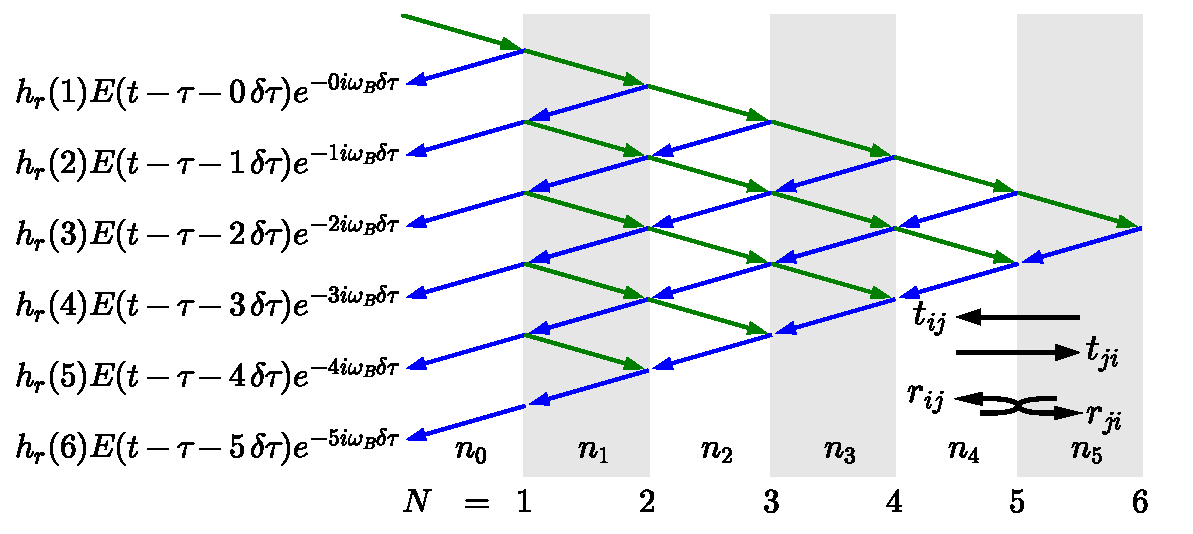
\includegraphics[width=0.8\linewidth]{Images/Chapter 2/discretised reflections.pdf}
    
    \caption{Illustration of the first 6 layers in the decomposition of an FBG in slabs and the contributions to the total reflected electric field. Each layers' transmission and reflection coefficients are indicated where $j = i+1$.}
    
    \label{fig:Slab_like_FBG_discretised}
\end{figure}
%
\par
%
In the past, all intra-layer reflections have been considered and summed over to produce expressions for the total reflection after a time delay $k \, \dt$ \cite{ghiringhelli2002time}. We consider a simpler model, initially applied to uniform FBGs whose average refractive index remains constant over the grating length. We demonstrate has the benefits of the mathematical tractability of the previously derived multiple Lorentzian model, while being capable of modelling the FBG reflection spectrum over a wider frequency spectrum. 
%
%
\section{Uniform FBG discretised reflection model derivation}
\label{sec:FBG_discretised_derivation}
%
We model the reflection response of the uniform FBG as a series partial reflections at boundaries equally spaced over the $N$ layers of the grating. The entire grating has a uniform refractive index $\neff$, while each boundary has an equal transmission coefficient $t$ and reflection coefficient $r$ at each boundary determined by the normalised refractive index variation $\dn = \dnbar/\neff$. Further, we consider only the dominant paths that undergo a single reflection at the $(k-1)^\text{th}$ layer. Therefore, a single reflection emerges from the uniform FBG after a time delay $\k \, \dt$. For this model to be physically valid, it must accurately reproduce the fundamental characteristics of FBGs—chiefly the total reflectivity $R$—while ensuring that the introduced parameters $r$ and $t$ have a concrete relationship with the physical parameters of FBGs. With these goals in mind, we begin by rewriting the total reflectivity $R$ in terms of the two key parameters of the discretised model, namely $\dn$ and $N$.
%
\begin{equation}
\label{eq:R_exact}
    R_\text{exact} = \tanh{\left(\frac{\pi}{2}\frac{N \dn}{1+\dn} \right) }
\end{equation}
%
The key observation then is that $R$ is approximated very well by
%
\begin{equation}
    \label{eq:R_approx}
    R_\text{approx} = 1 - \left( 1 - \dn\right)^{2N}
\end{equation}
%
as shown in Figure~\ref{fig:R_approximations}(a), where both expressions are plotted as a function of $\dn$ for different layer numbers $N$, demonstrating the excellent agreement. We now describe two interpretations of this model that produce expressions for $r$ and $t$ which recovers this approximation for $R$. 
%
\begin{figure}[!t]
    \centering
    
    \begin{overpic}[width=0.8\linewidth]{Images/Chapter 2/single_reflection_forwardbackward.pdf}
        \put(3,42){(a)}
    \end{overpic}\\[0.5em]
    \begin{overpic}[width=0.8\linewidth]{Images/Chapter 2/single_reflection_forward.pdf}
        \put(3,42){(b)}
    \end{overpic}
    
    \caption{Illustration of the first 6 layers in the decomposition of an FBG in slabs where only the final contribution due to reflection at the $k^{\text{th}}$ is considered for the $k^{\text{th}}$ delayed signal. Forward and backward transmission is considered in (a) while only forward transmission is considered in (b).}
    
    \label{fig:Slab_like_FBG_single}
\end{figure}
%
%
\subsection{Discretised reflection interpretation 1: Effective reflectivity}
%
Figure~\ref{fig:Slab_like_FBG_single}(a) illustrates this interpretation of the discretised FBG reflection. At each boundary, a signal propagating forward or backward is either transmitted or reflected. As previously discussed, intra-layer reflections that emerge from the grating after a time delay $k \, \dt$ are typically grouped together as $h_r(k)$. Here, we approximately account for all intra-layer reflections within $h_r(k)$ through the signal that is reflected at the $k^\text{th}$ layer, which has an identical time delay. Given that each of these signals are transmitted through $2(k-1)$ layers and reflected once, the reflection coefficient at the $k^{\text{th}}$ layer is given by
%
\begin{equation}
    \label{eq:hr2}
    h_r(k) = t^{2(k-1)}r
\end{equation}
%
We now require an $r$ and $t$ that recovers \eqref{eq:R_approx} when we sum over all reflections $h_r(k)$. Rewriting \eqref{eq:R_approx} as a sum,
%
\begin{align*}
    R_\text{approx} &= 1 - (1-\dn)^2 + (1-\dn)^2 - \dots - (1-\dn)^{2N-2} + (1-\dn)^{2N-2} - (1-\dn)^{2N}
    \\
    &= (1-(1-\dn)^2) \left( 1 + (1-\dn)^2 + \dots (1-\dn)^{2N-2} \right)
\end{align*}
%
Therefore,
%
\begin{equation*}
    R_\text{approx} \equiv \sum_{k=1}^{N} h_r(k) = (1-(1-\dn)^2)\sum_{k=1}^{N} (1-\dn)^{2(k-1)}
\end{equation*}
%
%
which is precisely the desired form for the sum of all reflected signals given by \eqref{eq:hr2} when we define
%
\begin{align*}
    t &\equiv 1-\dn
    \\
    r &\equiv 1-t^2
\end{align*}
%
We therefore have transmission and reflection coefficients $t$ and $r$ for this discretised reflection model which accurately describes the total FBG reflectivity, at least at its Bragg frequency. It is noted that the derived reflection coefficient $r$, which physically should be larger than what one would derive from optics equations to account for the intra-layer reflections that have been dropped, results in the relation
%
\begin{equation*}
    r + t = 1 + \dn - \dn^2 > 1 \; \forall \; \dn<1
\end{equation*}
%
demonstrating that modelled reflected signals account for many reflected signal, as expected. Although this representation can be used going forward, a slightly different viewpoint on this model produces expressions the authors find preferable.
%
\par
%
\subsection{Discretised reflection interpretation 1: Many mirrors}
%
While the previous interpretation 'lives' in the same modelling setup as previous approaches to discretised FBG reflections \cite{ghiringhelli2002time, capmany2007synthesis}, here we consider a more conceptual model for the FBG which is illustrated in Figure~\ref{fig:Slab_like_FBG_single}(b). We consider the reflected signals emerging from the front facet of the FBG after a time delay $k \, \dt$ as having effectively passed through $k-1$ partially reflective mirrors in a medium with refractive index $\neff$ before being reflected at the $k^\text{th}$, subsequently undergoing no further attenuation. Following this interpretation, the reflected signal at the $k^\text{th}$ layer has an effective reflection coefficient
%
\begin{equation}
    \label{eq:hr1}
    h_r(k) = t^{k-1}r
\end{equation}
%
We now follow the same procedure as done with the previous model, that is calculating n $r$ and $t$ that recovers \eqref{eq:R_approx} when we sum over all reflections $h_r(k)$. We have that \eqref{eq:R_approx} can be written as
%
\begin{equation*}
    R_\text{approx} = \sum_{k=1}^{N} h_r(k) = (1-(1-\dn)^2)\sum_{k=1}^{N} \left((1-\dn)^2\right)^{k-1}
\end{equation*}
%
Then,
%
\begin{align}
    \label{eq:tr}
    t &\equiv (1-\dn)^2
    \\
    r &\equiv 1-t
\end{align}
%
which then has the more preferable property that $r+t=1$. Given that both interpretations provide identical results, we use these expressions for the effective reflection $h_r(k)$ given by \eqref{eq:hr1} and $r$ and $t$ given by \eqref{eq:tr}. 
%
%
\subsection{LK equations under discretised FBG reflection}
We can, as has been done in several other analyses \cite{skenderas2024impact,skenderas2021feedback, li2012distributed,li2015chaotic,li2020stable}, then write the feedback $\eta F(t)$ as the convolution of the electric field with the impulse response
%
\par
%
\begin{align*}
    \eta F(t) &= \eta e^{-i C_p} E(t) \otimes \tilde{\rho}(t)
    \\
         &= \eta e^{-i C_p} E(t) \otimes \sum_{k=0}^{N-1} t^k r \delta(t-\tau-k\, \dt) e^{-i k \wB \dt}
    \\
         &=  \eta r e^{-i C_p} \sum_{k=0}^{N-1} t^k  E(t) \otimes \delta(t-\tau-k\, \dt) e^{-i k \wB \dt}
    \\
    \eta F(t) &=  \eta r e^{-i C_p} \sum_{k=0}^{N-1} t^k  E(t-\tau-k\, \dt) e^{-i k \wB \dt}
\end{align*}
%
where $e^{-i k \wB \dt}$ accounts for the phase accumulated while propagating through the FBG. This reduces the typical integral-based feedback term to a sum of discrete delays, resulting in a form for the LK equations given by 
%
\begin{equation}
\label{eq:LK_discretised}
    \begin{aligned}
        \frac{d E}{d t} & =(1+i \alpha) N(t) E(t)+\eta (1-t) e^{-i C_p} \sum_{k=0}^{N-1} t^k E(t-\tau-k\, \dt) e^{-i k \wB \dt} \\
        T \frac{d N}{d t} & =P-N(t)-(1+2 N(t))|E(t)|^2
    \end{aligned}
\end{equation}
%
where $\wB$ measures the grating's detuning from the laser free-running frequency, in the same way as with FOF.
%
\par
%
\begin{figure}[!t]
    \centering
    
    \hspace{0.04cm}
    \begin{overpic}[width=0.69\linewidth]{Images/Chapter 2/R discretised.pdf}
        \put(-5,40){(a)}
    \end{overpic}
    \hspace{0.1cm}
    \begin{overpic}[width=0.7\linewidth]{Images/Chapter 2/tau discretised.pdf}
        \put(-5,40){(b)}
    \end{overpic}
    
    \caption{A comparison between the exact total reflection and discretised total reflection is shown in (a), and the exact effective delay and discretised delay expectation is shown in (b) as functions of the normalised refractive index variation $\dn$ for varying $N \in [10,100,1000,10000]$.}
    
    \label{fig:R_approximations}
\end{figure}

%
To further justify the physical relevance of these values for $t$ and $r$ in this discretised reflection model, we can, similar to the Lorentzian approximation, compare the expected delay of the discretised reflections to the known effective delay. The effective time delay, given by \eqref{eq:taueff}, can be written in terms of the layer round-trip time $\dt = 2 \Lambda \neff/c$ as
%
\begin{equation}
    \tau_{eff} = \frac{R_\text{exact} \dt}{\pi \dn}
\end{equation}
%
The expected delay of the discretised reflections $E[\tau_{FBG}]$ is calculated as the weighted average of the delays of all the reflected signals, where the weights are the amplitudes of the reflected signals. Mathematically,
%
\begin{equation*}
    E[\tau_{FBG}] = \frac{r \sum_{k=1}^{N} t^{k-1} (k-1)\dt}{r \sum_{k=1}^{N} t^{k-1}}
\end{equation*}
%
The sum in the denominator is simply the sum of a geometric sequence, having a closed form
%
\begin{equation*}
    \sum_{k=1}^{N} t^{k-1} = \frac{1-t^N}{1-t}
\end{equation*}
%
while the sum in the numerator can be written in terms of a derivative w.r.t. $t$ of the numerator. That is,
%
\begin{equation*}
    \sum_{k=1}^{N} t^{k-1} (k-1) = t \, \partial_t \sum_{k=1}^{N} t^{k-1} = \frac{t(1-t^N)}{(1-t)^2} - \frac{N t^N}{1-t}
\end{equation*}
%
The effective delay then simplifies to
%
\begin{equation*}
    E[\tau_{FBG}] = \dt\left[ \frac{t}{1-t} - \frac{N t^N}{1-t^N} \right]
\end{equation*}
%
or alternatively,
%
\begin{equation*}
    E[\tau_{FBG}] = \dt\left[ \frac{t}{1-t} - \frac{N (1-R_\text{approx})}{ R_\text{approx}} \right]
\end{equation*}
%
Figure~\ref{fig:R_approximations}(b) plots both expressions for the total FBG time delay again as function of $\dn$ for different layer numbers $N$. Excellent agreement is seen in the total delay, as was the case with the total FBG reflectivity, particularly for low $\dn$ while diverging from the true effective delay as $\dn$ increases, further justifying these choices for $t$ and $r$. We note that this improved agreement in total time delay for lower $\dn$ is in direct contrast to the accuracy of the ratio of total reflectivities, which decreases in accuracy as the refractive index change decreases. Given the success of this FBG model in describing both total reflectivity and time delay to a good accuracy, we propose that \eqref{eq:LK_discretised} is a good approximation to the LK equations under FBG feedback, while being amenable to mathematical analyses available to the LK equation under COF. The key derived parameter $t$, present in \eqref{eq:LK_discretised} is calculated through \eqref{eq:R_approx}, as
%
\begin{equation}
\label{eq:discretised_t}
    t =  \big( 1-R \big) ^\frac{1}{N}
\end{equation}
%
%
\section{EGM modes of the discretised reflection model}
\label{sec:EGM_discretised}
%
\section{External grating modes of the Three Lorentzian model}
%
Given that the derived model is simply a coupled system of DDEs, we can, in the same vein as with ECMs of the COF laser and EFMs of the FOF laser, calculate the basic steady-state solutions of the system given by \eqref{eq:3Lorentzian_FBG_LK}. 
Such solutions are referred to as external grating modes (EGMs) herein. 
The ability to calculate these modes is a crucial advantage over other other systems modelling FBG feedback in semiconductor lasers as they provide much of the understanding in the structure of solutions and their stability \cite{rottschafer2007ecm}, while additionally allowing for enhanced model validation with the standard LK equations. 
Further, once the stable solutions have been calculated, they can be continued in parameters using specialised DDE numerical continuation software such as \texttt{DDE-BifTool}. 
The EGM modes have the form,
%
where $E_s, \w_s, N_s \in \mathbb{R}$. 
These solutions physically correspond to an electric field locked at a frequency $\w_s$ with constant amplitude $E_s$ at a constant inversion $N_s$. 
In this form $\w_s$ measures the mismatch from the solitary laser frequency. 
Inserting this ansatz into \eqref{eq:3Lorentzian_FBG_LK}, one can obtain an implicit equation for the EGM frequencies
%
We now come to a description of the transition of the EFM-components as the filter detuning D is varied. 
For D = 0 the bulge of the solution envelope is centred at the origin of the (xs, X)-plane; see Fig. 5(a). 
The associated single EFM-component is shown in Fig. 6(a). It corresponds to the single, continuous curve in Fig. 7(a). 
As D is increased, the bulge in the envelope moves along the diagonal towards the top-right of the (xs, X)plane; see Fig. 5(b). 
The EFM-component deforms in the (xs, Ns)-plane but it is still a single closed curve; see Figs. 6 and 7(b). 
It surrounds both the frequency of the filter xs = D and the free-running laser frequency xs = X = 0. 
As the filter detuning D is increased further, the envelope undergoes a saddle transition Ts at X = 0, which can be seen clearly in the Figs. 6(c) and 7(c) as a point where the curve self-intersects
%
The equations derived for the discretised reflection model very similar to the original LK equations given by \eqref{eq:LK} in that CW solutions are given by $(E(t), N(t)) = (E_s e^{i\w_s t}, N_s)$ without additional dimensions introduced by the feedback $F(t)$. We may solve this equation by expanding the complex exponentials into their real and imaginary components,
%
\begin{align*}
    i \w_s =(1+i \alpha) N_s + \eta (1-t) \big(&\cos{(\phi_{EC})} -i\sin{(\phi_{EC})}  \big) \times \\ &\left( \sum_{k=0}^{N-1} t^k \cos{(k\phi_{FBG})} - i \sum_{k=0}^{N-1} t^k \sin{(k\phi_{FBG})} \right)
\end{align*}
%
where $\phi_{FBG} = \dt(\wB + \w_s), \, \phi_{EC} = C_p+\tau \w_s$ are distinguished as the phases accrued in the EC and FBG, respectively. In this form, with the aid of identities
%
\begin{align*}
    \sum_{k=0}^{N-1} t^k \cos(k\phi_{FBG}) &= \frac{1 - t \cos(\phi_{FBG}) - t^N \cos(N\phi_{FBG}) + t^{N+1} \cos((N-1)\phi_{FBG})}{1 - 2t \cos(\phi_{FBG}) + t^2} \\
    \sum_{k=0}^{N-1} t^k \sin(k\phi_{FBG}) &= \frac{t \sin(\phi_{FBG}) - t^N \sin(N\phi_{FBG}) + t^{N+1} \sin((N-1)\phi_{FBG})}{1 - 2t \cos(\phi_{FBG}) + t^2}
\end{align*}
%
an implicit equation for the EGM frequencies $\w_s$ can be derived,
%
\begin{gather*}
    \begin{aligned}
\w_s = \frac{\eta (1-t) \sqrt{1 + \alpha^2}}{t^2 - 2 t  \cos(\phi_{FBG}) + 1} \Big[ - &\sin(\phi_{EC} + \arctan(\alpha)) \\
     +  t&\sin(\phi_{EC} + \arctan(\alpha) - \phi_{FBG}) \\
     + t^N&\sin(\phi_{EC} + \arctan(\alpha) + N \phi_{FBG})   \\
     -  t^{N+1}&\sin(\phi_{EC} + \arctan(\alpha) + (N-1) \phi_{FBG})
\Big]
\end{aligned}
\end{gather*}
%
The RHS can then be written as a single sine function, yielding
%
\begin{equation}
    \label{eq:discretised_ws}
    \w_s = -\eta (1-t) \sqrt{1+\alpha^2}\frac{S_N}{S} \sin{\left( \phi_{EC}+\arctan{(\alpha) + \Phi - \Phi_N } \right)}
\end{equation}
%
where
%
\begin{align}
    S &= \sqrt{1 - 2 t \cos{(\phi_{FBG}) + t^2}}
    \\
    S_N &= \sqrt{1 - 2 t^N \cos{(N\phi_{FBG}) + t^{2N}}}
    \\
    \Phi &= \arctan{\left( \frac{t \sin{(\phi_{FBG})}}{1 - t \cos{(\phi_{FBG})}} \right)} 
    \\
    \Phi_N &= \arctan{\left( \frac{t^N \sin{(N\phi_{FBG})}}{1 - t^N \cos{(N\phi_{FBG})}} \right)} 
\end{align}
%
We note that in the plane mirror limit, the front face of the FBG would reflect all incoming light, that is $ t = 0 \implies S = S_N = 1, \, \Phi = \Phi_N = 0$, yielding 
%
\begin{equation*}
    \w_s = - \eta \sqrt{\alpha^2 + 1} \sin{(C_p + \w_s \tau + \arctan(\alpha) })
\end{equation*}
%
which is precisely the well studied implicit ECM equation \cite{rottschafer2007ecm}. Given the solutions for $\w_s$, one can calculate $N_s$ and $E_s$ through
%
\begin{equation}
    N_s = -\eta (1-t) \frac{S_N}{S} \cos{\left( \phi_{EC} + \Phi - \Phi_N \right)}  
\end{equation}
%
\begin{equation}
    E_s = \sqrt{\frac{P - N_s}{1 + 2 N_s}}
\end{equation}
%
The envelope of $f$ is obtained by setting the sine term in \eqref{eq:discretised_ws} to $+1$ and $-1$.
%
\begin{equation}
    \label{eq:discretised_ws_envelope}
    \w_s = \mp \eta (1-t) \sqrt{1+\alpha^2}\frac{S_N}{S}
\end{equation}
while a curve of EGMs can also be derived by substituting the CW ansatz into \eqref{eq:LK_discretised}.
%
\begin{equation}
    \label{eq:discretised_Ns_curve}
    N_s(\w_s) = \frac{\alpha \w_s}{1+\alpha^2} \pm \frac{1}{1+\alpha^2}\sqrt{-\w_s^2 + (1+\alpha^2) \left(\eta (1-t) \frac{S_N}{S} \right)^2}
\end{equation}
%
\begin{figure}[!t]
    \centering
    
    \begin{overpic}[width=0.75\linewidth]{Images/Chapter 2/discretised_EGM_basecase.pdf}
        \put(3,78){(a)}
        \put(3,40){(b)}
    \end{overpic}
    
    \caption{Discretised reflection EGM solutions. EGM frequencies $\w_s$ correspond to intersections of $f_s(\w_s)$ (blue curve) and $g_s(\w_s)$ (green curve) in (a). The envelope of $f_s$, consisting of two black curves in (a), is obtained by setting the sine term in $f_s$ to $+1$ and $-1$. The EGM solutions and their curve in the $(\w_s, N_s)$-plane are shown in (b). The red dots correspond to a discrete set of EGMs while the black curve is given by \eqref{eq:discretised_Ns_curve}.}
    
    \label{fig:discretised_EGM_basecase}
\end{figure}
%
Lastly, while we can directly control the gratings reflectivity and detuning through $\eta$ (or $R$), and $\wB$, respectively, we can use the number of gratings $N$ to control the FBG bandwidth $\wz$ through \eqref{eq:wz} and \eqref{eq:discretised_t}.
%
\begin{equation}
    \label{eq:wztoN}
    \wz = \w_c \sqrt{\left( \frac{1 - (1 - R)^\frac{1}{2N}}{2} \right)^2 + \frac{1}{N^2}}
\end{equation}
%
\par
%
At this point, we have equations which can visualise the structure of the EGMs predicted by this discretised model which will help to fix the grating reflectivity $R$ and layer number $N$. We would like to study physically relevant EGMs of FBGs in parameter regions of interest. For 1550 nm light, the lasers angular frequency corresponds to $\w_c=1216\;\text{rad\,ps}^{-1}$. Then, to compare to the Lorentzian model, that nominally had $\wz = 0.1$, we must first determine the FBG parameters $(\wB, R, N)$ in \eqref{eq:wztoN}. We first prescribe the parameters of the laser and EC to the previously studied values $\tau = 121, \alpha = 3.5, \eta R = 0.0455, C_p = 0, T = 550, P = 0.186$ for COF \cite{heil2003delay}. It is then important to note that $\wz$ in the derived form of the LK equations is a dimensionless quantity normalised by the cavity lifetime $\tau_p$, which for these laser parameters is equal to $1.82 \,\text{ps}$, see Appendix~\ref{app:LK_approx} for details. Therefore, the angular frequency $\w_c$ is nondimensionalised to $\w_c=2211$ and then, beginning with a reflectivity $R = 0.5$ the grating number, calculated through \eqref{eq:wztoN}, is $N \approx 22440$. As was done with the Lorentzian FBG LK model, we visualise EGM frequencies $\w_s$ as intersections of the left- and right-hand sides of \eqref{eq:discretised_ws}, defined as $g(\w_s)$ and $f(\w_s)$, respectively, and project EGMs in the $(\w_s, N_s)$-plane. Figure~\ref{fig:discretised_EGM_basecase} demonstrates excellent agreement in the structure of EGMs within the main lobe of the FBG reflection spectrum with the Lorentzian model. Crucially, in addition to accurately modelling EGMs within the main lobe, potential intersections of side lobes of the reflection spectrum can be seen in (a). Before moving forward with an analysis of EGMs predicted by this model using these initial values of $R$ and $N$, we discuss two clear issues with the current solution structure. First, in contrast to the Lorentzian model, $f(\w_s)$ does not precisely equal zero at $\w_s = \wB \pm \wz$. These reflection zeros are of particular interest as stability fluctuations around these reflection zeros have been observed and thus including these features in the reflection spectrum is of significance for a physically accurate model. Second and perhaps most pressing is the number of grating layers $N$, corresponding to that number of additional terms in \eqref{eq:LK_discretised}, which is of great significance in numerical simulations. Even for very short gratings $\sim 1\text{mm}$, layers have lengths $\sim 0.5\mu\text{m}$ for 1550nm light in standard optical fibers, leading to 1000s of delay terms. Although this does not pose any issues when evaluating grating modes and the like with the analytical equations presented thusfar, numerical continuation would immediately be out of reach due to the large computational times associated with a system 1000s of delay terms, while numerical integration would require similar computational times to that of the convolution or Fourier transform based forms of the feedback term $F(t)$, nullifying many of the advantages that one would seek with the modelling simplifications presented up to now. 
%
\par
%
On the issue of the transmission zeros at $\pm n \wz, n \in \mathbb{N}$, we vary the envelope of \eqref{eq:discretised_ws} for varying $R$, while keeping the total feedback rate $\eta R$ constant, as shown in Figure~\ref{fig:discretised_EGM_envelope_variations}. Clearly, the desired transmission zeros are obtained for low values of $R$. The use use of very low values for $R$ does not pose any issues in practice, as one can rescale the feedback rate $eta$ so that $\eta R$ is at the desired level. We then note that in \eqref{eq:wz},
%
\begin{equation*}
    1-(1-R)^{-\frac{1}{2N}} \approx 0, R\ll1
\end{equation*}
%
Then, using $\w_c = 2\pi/\dt$, the location of reflection zeros, given by \eqref{eq:wztoN} simplifies to becomes
%
\begin{equation}
    \label{eq:wz_approx}
    \wz \approx \frac{2\pi}{\dt N}
\end{equation}
%
% \begin{figure}[!t]
%     \centering
%     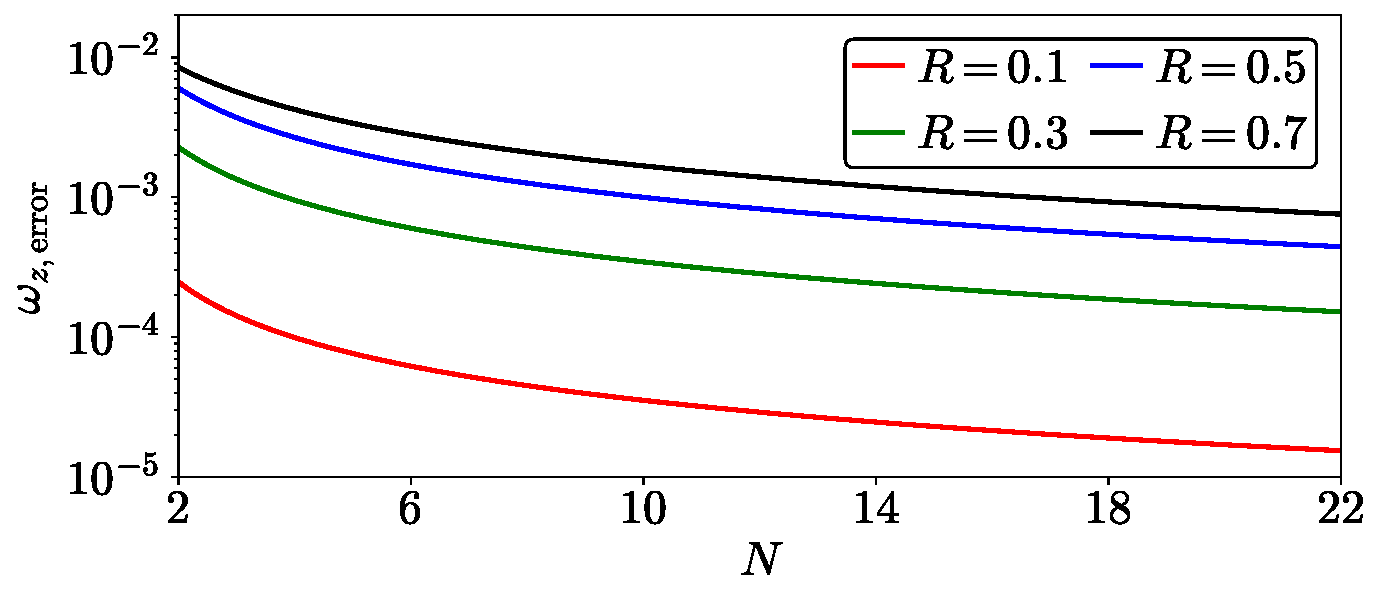
\includegraphics[width=0.72\linewidth]{Images/Chapter 2/wz_error.pdf}
%     \caption{Relative error between the exact and approximate values for $\wz$, given by \eqref{eq:wztoN} and \eqref{eq:wz_approx}, respectively, as a function of layer number $N$ for different total reflectivities.}
%     \label{fig:wz_error}
% \end{figure}
%
\begin{figure}
    \centering 
    
    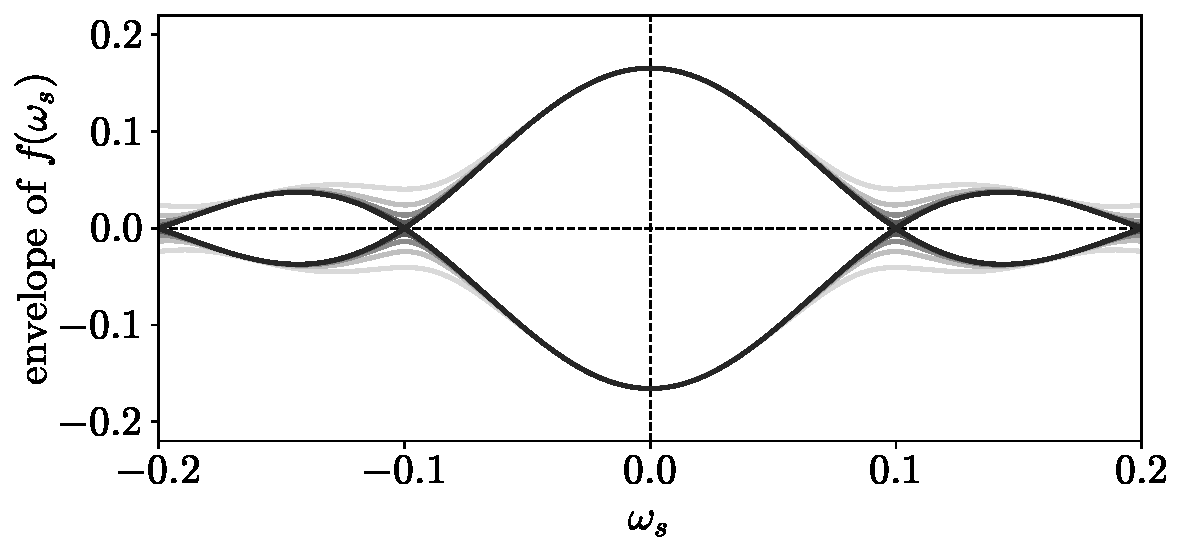
\includegraphics[width=0.75\linewidth]{Images/Chapter 2/discretised_EGM_envelope_variations.pdf}   
    
    \caption{figure}{Variation in the shape of the envelope of $f(\w_s)$ for $R \in [0.01, 0.2, 0.4, 0.6, 0.8]$ while keeping the effective feedback rate $\eta_{eff}$ constant.}
    
    \label{fig:discretised_EGM_envelope_variations}
\end{figure}
%
This simplification to the location of reflection zeros provides the key to addressing the issue of large number of delays $N$, which we seek to reduce while still obtaining identical dynamics. This approximation indicates that so long as the product $\dt N$ remains constant, the EGM bandwidth is unchanged. Note that this is equivalent to requiring that the total grating length remains constant, as $L = N \dt c/\neff$. An illustration of this is shown in Figure~\ref{fig:Low_N_gratings}. This tracks with physical intuition on gratings, as very short gratings ($L \ll 1$) act like mirrors, which are like filters with infinite bandwidth, while very long gratings ($L \gg 1$) produce a narrow bandwidth filtering response.
%
\begin{figure}[!t]
    \centering
    
    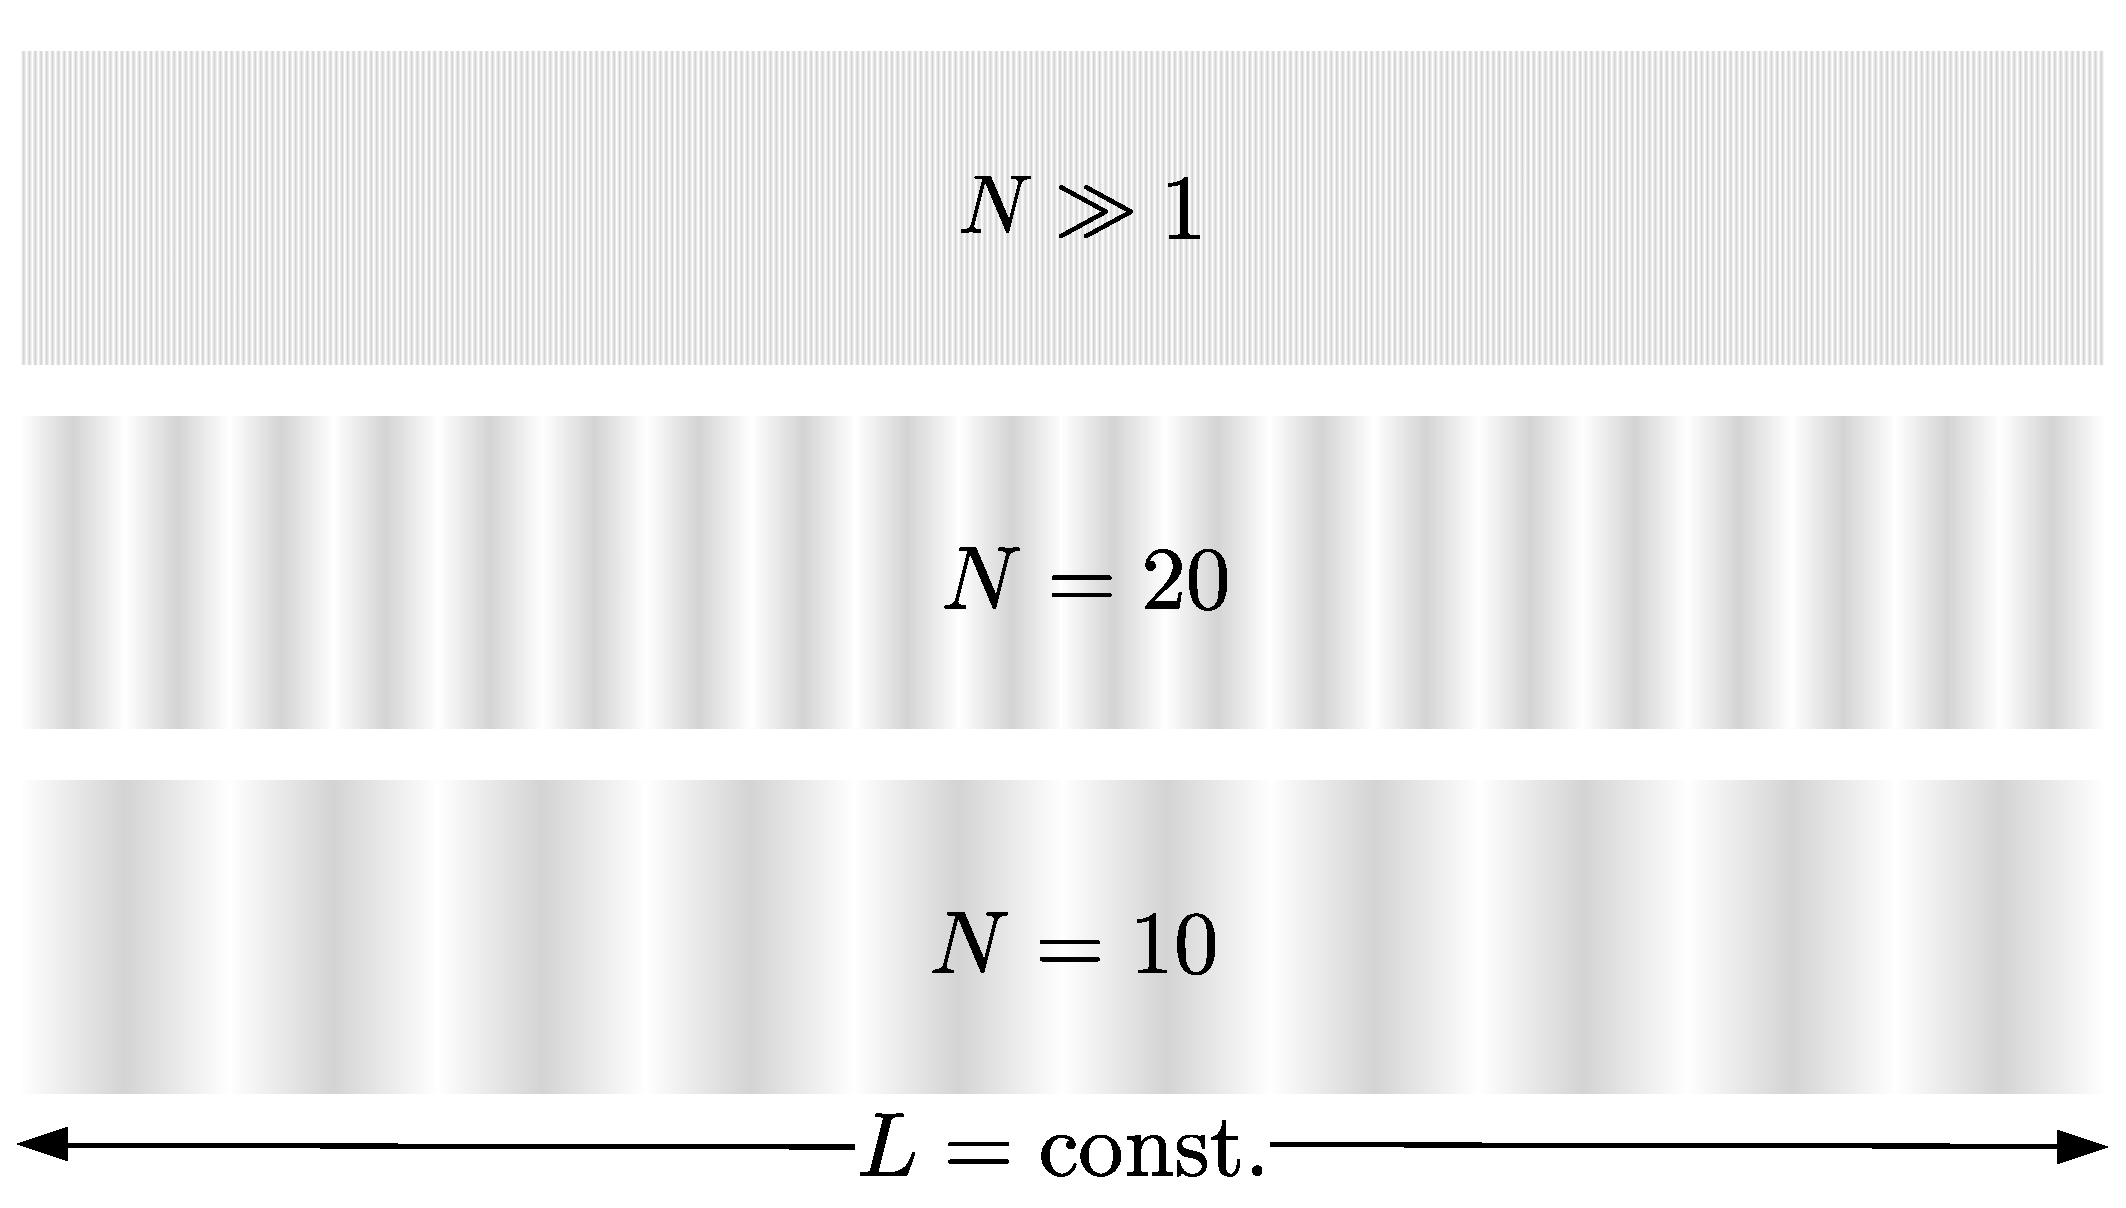
\includegraphics[width=0.6\linewidth]{Images/Chapter 2/Low N gratings.pdf}
    
    \caption{Illustrations of gratings with equal length but different layer numbers $N$, each providing near identical reflection zero locations $\wB \pm n\wz, \; n \in \mathbb{N}$.}
    
    \label{fig:Low_N_gratings}
\end{figure}
%
We therefore can calculate the required $\dt$ for a desired $\wz$ and $N$ through \eqref{eq:wz_approx}. The equivalence between different grating numbers is demonstrated in Figure~\ref{fig:discretised_EGM_accuracy}, where grating numbers $N \in [10, 22440]$ are used with near identical agreement. We therefore may select a layer number $N$ that is low enough to be amenable to standard numerical analyses such as continuation without encountering significant computational difficulties.
%
\begin{figure}[!t]
    \centering
    
    \begin{overpic}[width=0.75\linewidth]{Images/Chapter 2/discretised_EGM_accuracy.pdf}
        \put(4,78){(a)}
        \put(4,40){(b)}
    \end{overpic}
    
    \caption{Equivalence in EGM structure between different grating numbers $N \in [10, 22440]$ by keeping $N\dt$ constant.}
    
    \label{fig:discretised_EGM_accuracy}
\end{figure}
%
The key difference between using a low grating number is in the number of side lobes that are correctly modelled. Figure~\ref{fig:discretised_EGM_wide_view} plots the EGM solution curves over $\w_s \in [-20\wz, 20\wz]$ for $N = 10$ and $N = 22440$ while keeping $N\dt$ constant. It can be seen that when $N=10$, a main reflection lob appears after every $10\wz$, meaning that five side lobes are obtained before the model becomes completely non-physical. In contrast, the side lobes continue for the true grating number for 1550 nm light. Overall, a balance must be made between choosing an $N$ that is low enough so that the system is still amenable to analysis through integration and continuation, while not introducing non-physical features to the EGM structure over the parameter region being studied. To this end, we illustrate two undesirable situations that can occur for an insufficiently large $N$ in Figure~\ref{fig:discretised_EGM_minimumN}, which plots EGM solutions for $N=10$ for varying detuning $\wB$. The valid solution regions, corresponding to a frequency range of $\pm 5 \wz$, are plotted with opaque lines while the entire frequency region is plotted with semi transparent lines. The first case demonstrated in the left column illustrates how if the detuning $\wB$ becomes large enough, the valid portion can be completely detuned away from $\w_s=0$ as shown in the progression from (a1) to (b1). As the amplitude of side lobes will begin to increase again past this point as shown in (c1) (where they should continue to diminish) one could find larger EGM regions than is physically correct. This can be avoided by ensuring that over the parameter region being studied, $N$ is larger than $2{\w}_{B, \max}/{\w}_{z,\min}$. The second and perhaps more problematic case shown on the right column, occurs when repeated side lobes intersect the line $f(\w_s) = \w_s$. and the repeated main reflection lobes over the entire parameter region of interest. The first repetitions of the main lobe occur at $\w_s = \pm N \wz + \wB$, while each main lobe has a maximum at $\pm \eta \sqrt{1+\a^2}$. The line $f(\w_s)$ can therefore hit the first repeated main lobes at $\w_s = \pm \eta \sqrt{1+\a^2}$. For $\wB=0$ as shown in (a2), only valid regions of the EGM envelope intersect the line $f(\w_s)$, but as $\wB$ increases, the first repeated main lobe begins to intersect $f(\w_s)$ at $\w_s = \pm \eta \sqrt{1+\a^2}$ as shown in (b2), introducing invalid EGM components to the solution structure as $\wB$ is increased as shown in (c2). Note that detuning is not the only mechanism for which this can occur, for example, increasing the feedback rate $\eta$ in (b1) would increase the amplitude of the solution envelope and quickly cause intersections between the repeated main lobes and $f(\w_s)$. To guarantee these non-physical features are not introduced into the EGM structure, we therefore require the first repeated peaks to never be within $\w_s = \pm \eta \sqrt{1+\a^2}$, which can be ensured through
%
\begin{equation*}
    N \wz + |\wB| > \w_s = \eta \sqrt{1+\a^2}
\end{equation*}
%
Combining these two conditions, a lower bound on the grating number $N$ for a particular parameter region can then be prescribed as
%
\begin{equation}
    \label{eq:Nmin}
    N_\text{min} = \max \left\{ \left\lceil \frac{2|\wB|_{max}}{\w_{z,\min}} \right\rceil , \;\left\lceil \frac{|\wB|_{\max} + \eta_{\max} \sqrt{1+\a_{\max}^2}}{\w_{z,\min}} \right\rceil \right\}
\end{equation}
%
\begin{figure}[!t]
    \centering
    
    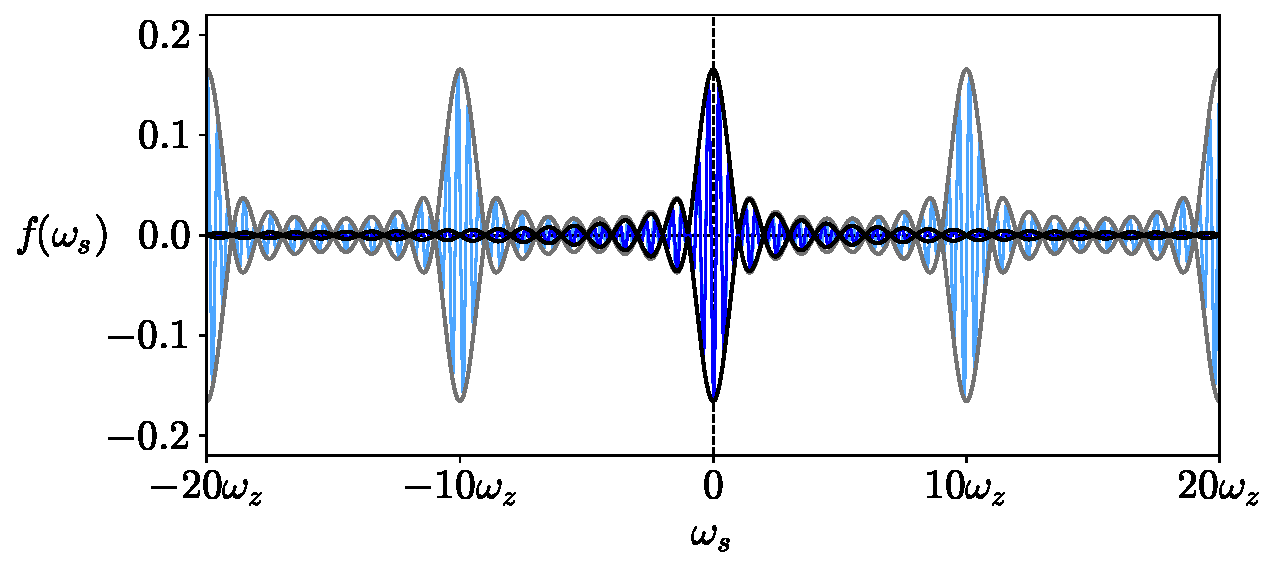
\includegraphics[width=0.75\linewidth]{Images/Chapter 2/discretised_EGM_wideview.pdf}
    
    \caption{EGM solutions over a wide frequency range $\w_s \in [-20\wz, 20\wz]$ for two different grating numbers $N = 10$ and $N = 22440$ while keeping $N\dt$ constant.}
    
    \label{fig:discretised_EGM_wide_view}
\end{figure}
%
\begin{figure}[!t]
    \centering
    
    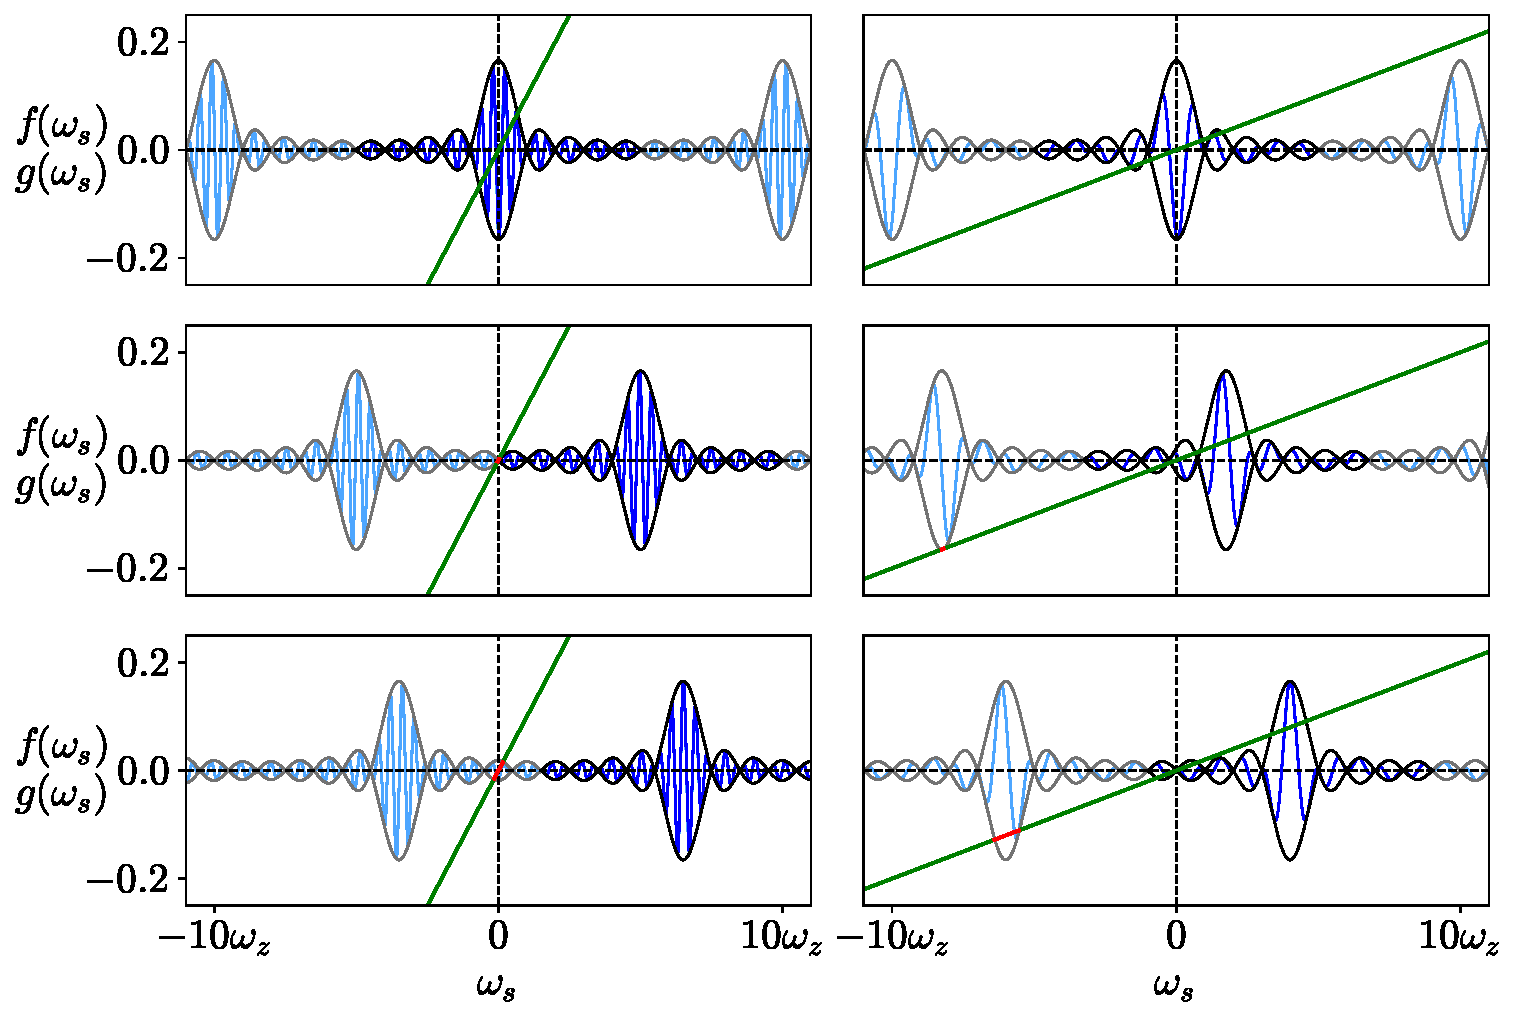
\includegraphics[width=0.94\linewidth]{Images/Chapter 2/discretised_EGM_minimumN.pdf}
    
    \caption{EGM solutions for varying detuning $\wB$ with $\wz=0.1$ (left) and $\wz=0.02$ (right) and $N=10$ in both cases. Valid region solution regions are plotted with opaque lines while the entire frequency region is plotted with semi transparent lines.}
    
    \label{fig:discretised_EGM_minimumN}
\end{figure}
%
While a low reflectivity $R$ does provide the desired transmission zeros, the relative errors in both total reflectivity $R_\text{error}$ and delay $\tau_\text{error}$ are larger compared to larger total reflectivities. This is demonstrated in Figure~\ref{fig:NR_Selection}, which visualises the combined relative errors $R_\text{error}$ and $\tau_\text{error}$ using the Euclidean metric $\| R_\text{error}, \tau_\text{error} \|_{_2} = \sqrt{R_\text{error}^2 + \tau_\text{error}^2}$. For the choice $N=10$, a total reflectivity $R_\text{approx} = 0.75$ would provide a lower combined error of 4\% as shown in (a) compared to the $R_\text{approx} = 0.1$ which has a combined error of 19\%. As the ability to effectively describe and analyse transmission zeros of FBGs is of great interest, this increase in combined error, which is still relatively low from a modelling perspective, is a an acceptable trade-off.
\begin{figure}
    \centering
    
    \begin{overpic}[width=0.8\linewidth]{Images/Chapter 2/NR Selection large R.pdf}
        \put(0,34){(a)}
    \end{overpic}\\[0.5em]
    \begin{overpic}[width=0.8\linewidth]{Images/Chapter 2/NR Selection low R.pdf}
        \put(0,40){(b)}
    \end{overpic}
    
    \caption{figure}{Combined relative errors of FBG total reflectivity $R_\text{error}$ and delay $\tau_\text{error}$ as a function of the grating number $N$ and normalised refractive index variation $\dn$. Level sets of constant total reflectivity $R_\text{approx}$ are overlayed in white. In (a), the square marker at $(N,\dn) = (10, 0.07)$, corresponding to an $R_\text{approx} = 0.75$ has a combined error of 4\% while in (b), the marker at $(N,\dn) = (10, 0.0055)$, corresponding to an $R_\text{approx} = 0.1$ has a combined error of 19\%.}
    
    \label{fig:NR_Selection}
\end{figure}
%
\par
%
Note then, that the final grating parameter $\dt$, which determines the grating length $L$, controls the grating bandwidth. The effective feedback rate is defined as $\eta_{eff} \equiv \eta R$. We can now compare the two derived models describing FBG distributed feedback. The first of which derived directly from the FBG reflection spectrum $\rho(\w)$ using Lorentzian distributions, and the present model, approximating the FBG impulse response $\tilde{\rho}(t)$. We compare EGM solutions of both models using identical parameters in Figure~\ref{fig:discretised_3Lorentzian_EGM_comparison} where results obtained by the discretised reflections model are plotted with solid lines and round markers, while results obtained by the Lorentzian model are plotted with dashed lines and square markers. Remarkable agreement between these models can be seen, in spite of their independent derivations. The nulls of the envelopes of $f(\w_s)$ in both cases agree precisely, while their values at $\w_s=0$ only show slight disagreement, due to the error in total reflectivity in the discretised reflection model for $R=0.01$. Further, both models predict 11 EGMs with excellent agreement in their locations. As the Lorentzian model has a more physically concrete derivation, this gives strong evidence as to the physical relevance of the discretised reflection model, while having the added benefit of modelling side lobes of the reflection spectrum. 
%
\begin{figure}[!t]
    \centering
    
    \begin{overpic}[width=0.75\linewidth]{Images/Chapter 2/discretised_threeLorentzian_EGM_comparison.pdf}
        \put(4,78){(a)}
        \put(4,40){(b)}
    \end{overpic}
    
    \caption{EGM solutions of the Lorentzian and discretised reflection model using identical parameter values. Results obtained by the discretised reflections model are plotted with solid lines and round markers, while results obtained by the Lorentzian model are plotted with dashed lines and square markers.}
    \label{fig:discretised_3Lorentzian_EGM_comparison}
\end{figure}
%
\par
%
\section{Comparison to previously studied FBG feedback models}
\label{sec:model_comparison}
%
Given the excellent agreement in ECMs confined to the main lobe between the three Lorentzian model and the discretised reflection model, we now compare agreement in solution structure and system dynamics between the discretised reflection model and the various approaches to modelling the feedback term $F(t)$ within the LK equations in the literature. This section demonstrates the excellent agreement this discretised model demonstrates with significantly less computational effort, while portraying several analysis techniques available to this system that is not possible with previously studied forms of FBG feedback. 
%
%
\subsection{EGM Accuracy}
\label{subsec:naumenko}
A considerably more complex system presented by Naumenko \textit{et al.} in \cite{naumenko2003characteristics} considers the feedback term $F(t)$ in the form of \eqref{eq:multiple_EC} that is, as the inverse Fourier transform of the product of the time delayed electric field in the spectral domain $\mathcal{F}[E(t-\tau)](\w)$ and the grating reflection spectrum $\rho(\w)$. The model additionally considers nonlinear gain and frequency chirp due to thermal effects when the injection current is changed. Ignoring these additional effects, and making suitable approximations, the system simplifies to the derived discretised reflection system as shown in Appendix~\ref{sec:multiple_EC_nondim} with parameter values $(\a, P, T, \tau, C_p) = (4, 0.5, 123, 512, 0)$, and varying grating parameters $\eta$, $\wB$, and $\wz$.
%
\par
%
EGMs were calculated with the help of Green functions through an involved mathematical procedure, as opposed to deriving closed form analytical equations. As discussed in the introduction, they identified `satellite' EGMs, separated from the central EGM envelope by the zeros of the main lobe by varying both grating bandwidth $\wz$ and detuning $\wB$.
%
\begin{figure}[!t]
    \centering

    \begin{minipage}[t]{0.43\textwidth}
        \vspace*{0pt}
        \begin{overpic}[width=\linewidth]{Images/Chapter 2/rB_003_annotated.pdf}
            \put(4,96){(a1)}
            \put(4,45){(b1)}
        \end{overpic}
    \end{minipage}
    \hspace{2em}
    \begin{minipage}[t]{0.4\textwidth}
        \vspace*{0em}
        \begin{overpic}[width=\linewidth]{Images/Chapter 2/Naumenko_rB003.pdf}
            \put(0,68){(a2)}
        \end{overpic}
        \vskip 1.0em
        \hspace{0.0em}
        \begin{overpic}[width=0.97\linewidth]{Images/Chapter 2/Naumenko_EGM_rB003.pdf}
            \put(-3,77){(b2)}
        \end{overpic}
    \end{minipage}
   
    \caption{A comparison between EGMs in the multiple reflection (left) and discretised FBG (right) models in the frequency-intensity domain for varying grating bandwidth and zero detuning. The curves in panels (a1) and (a2) illustrate the FBG frequency responses. A constant reflectivity of $R=0.0316$ yields a nondimensionalised effective feedback rate $\eta=0.085$ while Bragg grating reflection zeros at 1/3, 4/3, and 20/3 GHz yield nondimensionalised reflection zero locations $\wz=0.016\pi, \; 0.064\pi, \; 0.32\pi$. The EGMs in panels (b1) and (b2) corresponding to these respective bandwidths are plotted with circles $(\circ)$, diamonds $(\diamond)$ and squares $(\square)$, while the MGM in each case is plotted indicated by a $\times$.}
    
    \label{fig:Naumenko_rB003}
\end{figure}
%
\begin{figure}[!t]
    \centering
    
    \begin{minipage}[t]{0.45\textwidth}
        \vspace{0pt}
        \begin{overpic}[width=\linewidth]{Images/Chapter 2/rB_02_annotated.pdf}
            \put(4,94){(a1)}
            \put(4,46){(b1)}
        \end{overpic}
    \end{minipage}%
    \hspace{1em}
    \begin{minipage}[t]{0.4\textwidth}
        \vspace{0.5em}
        \begin{overpic}[width=\linewidth]{Images/Chapter 2/Naumenko_rB02.pdf}
            \put(0,69){(a2)}
        \end{overpic}
        \vskip 0.5em
        \hspace{0.2em}        
        \begin{overpic}[width=0.96\linewidth]{Images/Chapter 2/Naumenko_EGM_rB02.pdf}
            \put(-3,79){(b2)}
        \end{overpic}
    \end{minipage}

    \caption{A comparison between EGMs in the multiple reflection (left) and discretised FBG (right) models in the frequency-intensity domain for a detuned FBG. A reflectivity of $R=0.224$ yields a nondimensionalised effective feedback rate $\eta=0.600$ while a Bragg grating reflection zero at 10/3 GHz yields nondimensionalised reflection zero location $\wz=0.16\pi$. Finally, a detuning of 8 GHz corresponds to $\wB=0.384\pi$.}
    
    \label{fig:Naumenko_rB02}
\end{figure}
%
Figures~\ref{fig:Naumenko_rB003} and \ref{fig:Naumenko_rB02} compare results obtained by both the multiple EC reflection FBG feedback and discretised FBG models for varying grating reflectivity, bandwidth and detuning. In order to to obtain valid EGM solutions, for both parameter sets, $N=10 > N_\text{min}=7$ was used. Solutions are projected in the frequency-intensity plane where $I = |E|^2$, in contrast to the usual projection in the inversion-frequency plane, causing an inversion of the cavity modes about the frequency axis. The photon lifetime $\tau_p=24\,\text{ps}$ was used to convert grating bandwidths in Hz to their nondimensionalised $\wz$ form. Clearly, excellent agreement in the mode structure is achieved, in particular for the low feedback rate case. Firstly, considering no detuning, low feedback and varying bandwidths as is the case in Figure~\ref{fig:Naumenko_rB003}, for a wide bandwidth of the Bragg reflector (in this case, a main lobe width of 40/3 GHz or $2\wz=0.64\pi$ in nondimensionalised form), EGMs lie on a closed curve, resembling a COF ECM structure, as expected. The MGM (mode with highest power) is located for near the edge of the left side of the closed curve, indicated by an '$\times$' in the figure. As the FBG bandwidth is decreased, the number of EGMs decreases, and the EGM solution curve and MGM narrows as they are confined to within the bandwidth of the main lobe, in agreement with results obtained from Sections~\ref{sec:EGM_Lorentzian} and \ref{sec:EGM_discretised} and with results obtained for a single Lorentzian filter \cite{yousefi1999dynamical}. Further narrowing the filter bandwidth introduces satellite EGMs, indicated with triangles, due to the side lobes of the FBG reflection spectrum. It is noted that this effect does not occur in the single Lorentzian filter for zero detuning. At this point, the MGM as nearly at the Bragg frequency, in agreement with physical intuition. Increasing the feedback rate considerably, and detuning the FBG from the laser's free-running frequency, as shown in Figure~\ref{fig:Naumenko_rB02}, also detune the EGM modes, and split the modes into three disjoint curves, corresponding to the main lobe and two side lobes nearest to the laser's free-running frequency. This splitting of solution curves was similarly observed for the single Lorentzian filter \cite{yousefi1999dynamical}, but at most two disjoint curves can be formed \cite{green2006mode}, while in this case already three distinct solution curves are present. Significant distortion in the EGM structure along the intensity axis can be seen for the discretised reflection case compared to the Multiple EC reflection model, which can be attributed to the lack of a gain suppression factor in this model in this simplified model. In any case, excellent agreement in the locations of the EGM components, MGM, and number of EGM solutions demonstrates the ability of the discretised reflections model to capture the solution structure of FBG feedback.
%
\par
%
% \begin{figure}[!t]
%     \centering
    
%     \begin{overpic}[width=0.8\linewidth]{Images/Chapter 2/Li_P1_local_minima.png}
%         \put(4,78){(a1)}
%         \put(54,78){(a2)}
%     \end{overpic}
%     \vskip 0.5cm
%     \hspace{-0.2cm}
%     \begin{overpic}[height=0.3\linewidth]{Images/Chapter 2/Li_chaos_FBG_extrema_001eta02.pdf}
%         % \put(4,78){(b1)}
%     \end{overpic}   
%     \hspace{0.0cm}
%     \begin{overpic}[height=0.3\linewidth]{Images/Chapter 2/Li_chaos_mirror_extrema_001eta02.pdf}
%         % \put(4,78){(b2)}
%     \end{overpic}    
%     \caption{}
%     \label{fig:P1_comparison}
% \end{figure}
%
%
\subsection{Stability Fluctuations}
\label{subsec:lichaos_skenderas}
%
%
It is important to note that while the locations of zeros in the discretised model are uniform, is only the case for FBGs which have relatively low reflectivities, see Figure~\ref{fig:uniform_spectra_varykL}. For this, re
%

\begin{figure}[p]
    \centering
    
    \begin{minipage}[t]{0.44\textwidth}
        \begin{overpic}[width=\linewidth]{Images/Chapter 2/Li_chaos_heatmap.png}
            \put(-2,85){(a)}
        \end{overpic}
    \end{minipage}%
    \hspace{0.5em}
    \begin{minipage}[t]{0.46\textwidth}
        \raisebox{-1em}{%
            \begin{overpic}[width=\linewidth]{Images/Chapter 2/discretised_Lichoatic_wBeta_comparison.pdf}
                \put(-2,85){(b)}
            \end{overpic}
        }
    \end{minipage}
    \\
    \begin{minipage}[t]{0.9\textwidth}
        \vspace{0.2em}
        \begin{overpic}[width=\linewidth]{Images/Chapter 2/discretised_Lichoatic_wBeta_xy_forwardbackward_comparison_lyapunov.pdf}
            \put(-2,68){(c)}
        \end{overpic}
    \end{minipage}

    \caption{Comparison between two parameter dynamical mappings of output intensity for a convolved FBG feedback form of $F(t)$ \cite{li2012distributed,li2015chaotic,li2020stable} (a) and the discretised FBG feedback form of $F(t)$ in the parameter space of feedback strength ($\xi_f$ in (a) and equivalent $\eta$ in (b)) and grating detuning frequency ($\Delta f$). In (a), the laser output intensity is stable (white), period-one oscillatory (red), quasi-periodic pulsating (gray), period-doubled oscillatory (yellow), and chaotic (black). In (b), the laser output is in steady-state (white), period-one oscillatory (red), period-two (yellow), and period 3 to very large period in a gradient from grey to black. In (c) parameter sweeps are performed in all four directions, with Hopf bifurcations of steady state EGMs overlayed}
    
    \label{fig:Li_chaos}
\end{figure}
%
\par
%
Finally, we compare our model to the most recent work on semiconductor lasers under FBG feedback by \Skenderas \textit{ et al.} \cite{skenderas2021feedback,skenderas2024impact}. In contrast to the previous two models, where nondimensionalisations and approximations were required before direct comparisons could be made, the form of the equations analysed mirror the equations presented in this work, using parameter values $(\a, P, T, \tau) = (3, 1, 1000, 1000)$, except for the use of a convolution feedback term $F(t)$ of the form \eqref{eq:convolution}. The results presented by \Skenderas \textit{ et al.} therefore serve as the most suitable basis for comparisons in the accuracy of the derived discretised model. Given the complexity of analysing the LK equations under FBG feedback using a convolution term, the results presented, like those previously studied, are obtained solely through analysis of time series obtained through numerical integration. The main focus of their analysis is in characterising the interplay between the lasers relaxation oscillations (ROs) and the FBG reflection zeros as a function of feedback rate $\eta$ and grating bandwidth $\wz$ for varying feedback phase $C_p$ and grating detuning $\omega_B$. 

ROs are the most typical type of oscillation that one would expect in semiconductor lasers. They are damped intensity fluctuations that occur when the laser transitions between steady states, typically after a sudden change in injection current, and arise from the dynamic interplay between photon density and carrier density in the laser cavity. When the carrier population is perturbed, it overshoots the steady-state value, causing oscillations in output power at a characteristic frequency known as the relaxation oscillation frequency $\w_\text{RO}=\sqrt{2P/T}$, which form the dominant side lobes either side of the centre frequency in the Fourier spectrum of a semiconductor laser. Exciting the ROs of a laser can lead to a more unstable laser, and therefore one would expect that lower amount of feedback would cause the laser to transition from steady output to oscillatory and then more unstable outputs. 

The strategy employed by the authors to observe They do this by tracking the Hopf bifurcation of the steady state of the laser in the $(L_\text{FBG},\eta)$-plane, where the grating length $L_\text{FBG}$ can be used to control the grating bandwidth $\wz$ as discussed in \ref{sec:EGM_discretised}. As discussed in \ref{sec:FBG}, varying the grating length also changes the grating reflectivity, therefore, when using this model, grating parameters must be simultaneously varied to solely vary its bandwidth. This is not an issue with the discretised reflections model as bandwidth $\wz$ and thus length $L_\text{FBG}$ can be varied independent of reflectivity using \ref{eq:wz_approx}
%
\begin{equation}
    L [\text{m}] \approx \frac{\pi c \tau_p}{\wz \neff} 
\end{equation}
%
where $\tau_p$ is the photon lifetime used to rescale time in this form of the LK equations as discussed in Section~\ref{sec:EGM_discretised}.
%
\par

%
\begin{figure}[!t]
    \centering   
    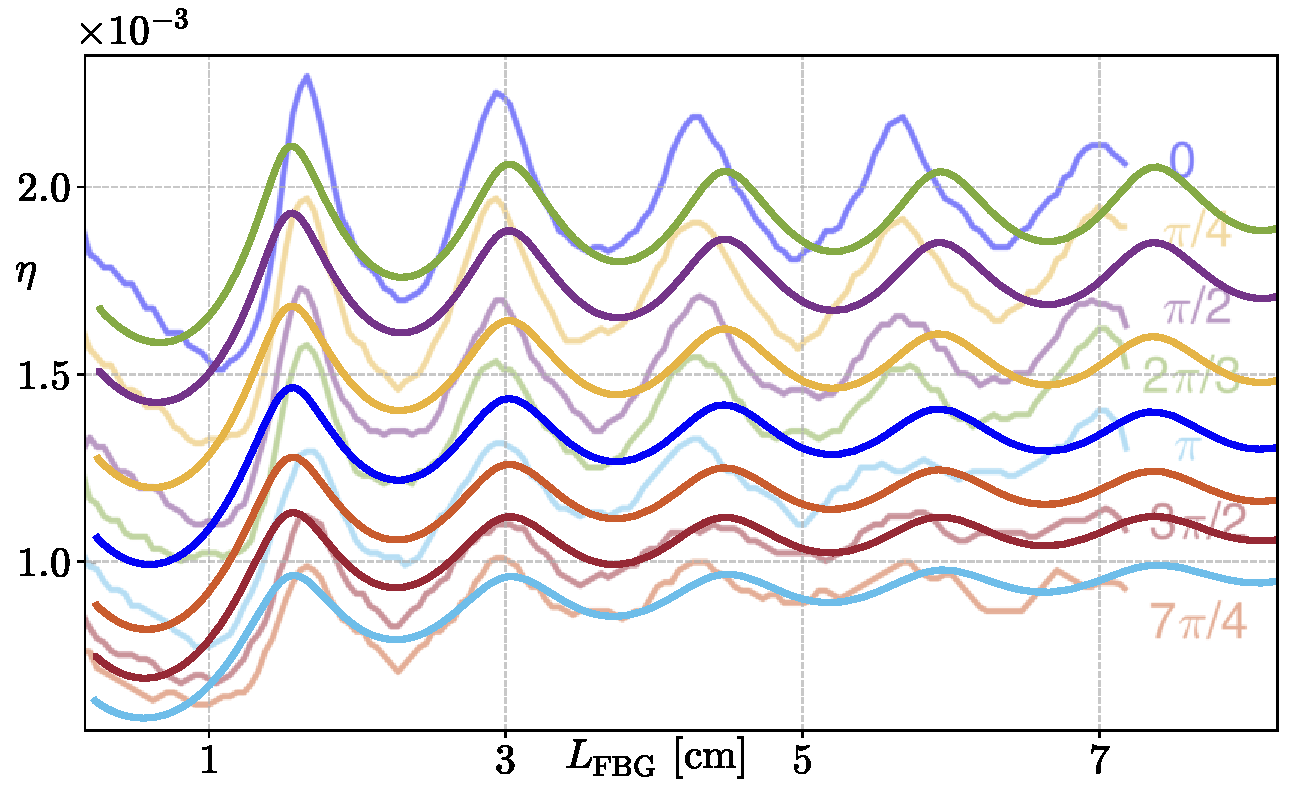
\includegraphics[width=0.75\linewidth]{Images/Chapter 2/discretised_Skenderas_wzeta_Cpcomparison_N20.pdf}    
    \caption{The evolution of Hopf bifurcation tracking the stability fluctuations as a function of $L_\text{FBG}$ at zero detuning for different values of the feedback offset phase $C_p$ equal to $0$ (blue), $\pi /4$ (yellow), $\pi/2$ (violet), $2\pi/3$ (green), $\pi$ (cyan), $3\pi/2$ (maroon), and $7\pi/4$ (orange).}
    \label{fig:Skenderas_Hopf_Cpvars}
\end{figure}
%
\begin{figure}[p]
    \centering
    
    \begin{minipage}[t]{0.45\textwidth}
        \begin{overpic}[width=\linewidth]{Images/Chapter 2/discretised_Skenderas_wBeta_image.pdf}
            \put(-5,80){(a)}
        \end{overpic}
    \end{minipage}%
    \hspace{0.5em}
    \begin{minipage}[t]{0.45\textwidth}
        \raisebox{0em}{%
            \begin{overpic}[width=\linewidth]{Images/Chapter 2/discretised_Skenderas_wBeta_comparison.pdf}
                \put(-5,80){(b)}
            \end{overpic}
        }
    \end{minipage}
    \\
    \begin{minipage}[t]{0.94\textwidth}
        \begin{overpic}[width=\linewidth]{Images/Chapter 2/discretised_Skenderas_wBeta_xy_forwardbackward_comparison.pdf}
            \put(-2,65){(c)}
        \end{overpic}
    \end{minipage}

    \caption{Comparison between two parameter dynamical mappings of output intensity for a convolved FBG feedback form of $F(t)$ \cite{li2012distributed,li2015chaotic,li2020stable} (a) and the discretised FBG feedback form of $F(t)$ in the parameter space of feedback strength ($\xi_f$ in (a) and equivalent $\eta$ in (b)) and grating detuning frequency ($\Delta f$). In (a), the laser output intensity is stable (white), period-one oscillatory (red), quasi-periodic pulsating (gray), period-doubled oscillatory (yellow), and chaotic (black). In (b), the laser output is in steady-state (white), period-one oscillatory (red), period-two (yellow), and period 3 to very large period in a gradient from grey to black. In (c) parameter sweeps are performed in all four directions, with Hopf bifurcations of steady state EGMs overlayed}
    
    \label{fig:Skenderas_wBeta}
\end{figure}
%


% !TeX root = ../main.tex
\section*{Conclusions and future developments}
\label{sec:conclusions}%
A final chapter containing the main conclusions of your research/study
and possible future developments of your work have to be inserted in this chapter.


% =======================
% Acknowledgments (optional)
% =======================
\begin{acknowledgments}
We acknowledge ...
\end{acknowledgments}

% =======================
% Appendices (optional, modular)
% =======================
\appendix
% !TeX root = ../main.tex
\section{Nondimensionalisation of the original LK Equations}
\label{sec:LK_nondim}
%
\let\cleardoublepage\origcleardoublepage
%
To model the dynamics of a semiconductor laser with optical feedback from an external cavity, we use the well-known \textbf{Lang-Kobayashi equations} \cite{lang1980external}. These delay differential equations describe how the complex electric field \( E(s) \) of the laser and the carrier inversion \( N(s) \) evolve in time under the influence of both intrinsic gain mechanisms and delayed feedback. In dimensionalised form, the equations are written as:
%
\label{eq:dimensionalised_LK}
\begin{gather}
\begin{aligned}
\frac{d E}{d s} &= \frac{1}{2} G_{\mathrm{M}0}(1 + i \alpha) \left[N(s) - N_N\right] E(s) + \kappa_0 e^{-i C_p} F(s, \tau_0)\\
\frac{d N}{d s} &= J_0 - \gamma_0 N(s) - \left[\Gamma_{\mathrm{M}0} + G_{\mathrm{N}0}(N(s) - N_N)\right] |E(s)|^2.
\end{aligned}
\end{gather}
%
The physical parameters in these equations are defined as follows:
\begin{itemize}
  \item \( \alpha \): linewidth enhancement factor
  \item \( \gamma_0 \): carrier decay rate
  \item \( \Gamma_{\mathrm{M}0} \): cavity decay rate
  \item \( \kappa_0 \): feedback strength
  \item \( \tau_0 \): external round-trip delay
  \item \( G_{\mathrm{M}0}, G_{\mathrm{N}0} \): small-signal gain coefficients
  \item \( J_0 \): pump current
  \item \( N_N \): inversion at threshold
\end{itemize}
%
\par
%
To simplify the equations and reduce the number of parameters, we introduce scaled variables:
%
\[
X = \frac{G_{\mathrm{M}0}}{2 \gamma_p}(N - N_N), \quad A = \sqrt{\frac{G_{\mathrm{N}0}}{2 \gamma_0}} E,
\]
where \( \gamma_p = \Gamma_{\mathrm{M}0} G_{\mathrm{M}0} / G_{\mathrm{N}0} \) is a rescaled photon lifetime. Rescaling time via \( t = \gamma_p s \), the Lang-Kobayashi equations become:
%
\[
\begin{gathered}
\frac{d A}{d t} = (1 + i \alpha) A X + \eta e^{-i C_p} F(t,\tau) \\
T \frac{d X}{d t} = P - X - (1 + 2X)|A|^2
\end{gathered}
\]
%
The transformed parameters are defined as:
%
\begin{itemize}
  \item \( P = \frac{G_{\mathrm{M}0}}{2 \gamma_p \gamma_0}(J_0 - \gamma_0 N_N) \): pumping rate above threshold
  \item \( T = \frac{\gamma_p}{\gamma_0} \): ratio of photon to carrier lifetime
  \item \( \eta = \frac{\kappa_0 G_{\mathrm{N}0}}{G_{\mathrm{M}0} \Gamma_{\mathrm{M}0}} \): normalized feedback strength
  \item \( \tau = \gamma_p \tau_0 \): rescaled external delay
\end{itemize}
%
The dimensionalised parameter values used are:
%
\[
\alpha = 3.5, \quad \gamma_0 = 1.0 \times 10^9, \quad \Gamma_{\mathrm{M}0} = 0.55 \times 10^9, \quad \kappa_0 = 25.0 \times 10^9,
\]
\[
\tau_0 = 0.22 \times 10^{-9}, \quad G_{\mathrm{M}0} = 50.0, \quad G_{\mathrm{N}0} = 0.05, \quad J_0 = 8.0 \times 10^9, \quad N_N = 5.0.
\]
Therefore, $\gamma_p = 5.5 \times 10^{11}$ resulting in nondimensionalised parameter values,
\[
\a = 3.5, \quad P = 0.136, \quad T = 550, \quad \eta = 0.0455, \quad \tau = 121.
\]
%
It is noted that one can get from this nondimensionalised time to second by multiplying by the factor $\tau_p = 1/\gamma_p = 1.82 \times 10^{-12}\,\text{s}$.
%
%
\section{Multiple EC reflection FBG LK model conversion}
\label{sec:Li_chaos_nondim}
%
The form of the equations analysed by Li \textit{et. al} are given by
%
\begin{equation}
\left\{\begin{array}{l}
\displaystyle \frac{d a}{d t}=\frac{1-i b}{2}\left[\frac{\gamma_{c} \gamma_{n}}{\gamma_{s}} \tilde{n}-\gamma_{p}\left(|a|^{2}-1\right)\right] a+\gamma_{c} \xi_{f} e^{i \theta}\left[r(t) e^{-i \Delta \Omega t}\right] * a\left(t-\tau_\text{RT}\right) \\
\displaystyle \frac{d \tilde{n}}{d t}=-\left(\gamma_{s}+\gamma_{n}|a|^{2}\right) \tilde{n}-\gamma_{s} \tilde{J}\left(1-\frac{\gamma_{p}}{\gamma_{c}}|a|^{2}\right)\left(|a|^{2}-1\right)
\end{array}\right.
\end{equation}
%
we first make a change of notation:
%
\begin{equation*}
\left\{\begin{aligned}
a & =E \\
\tilde{n} & =N \\
F(t) & =\left[r(t) e^{-i \Delta \Omega t}\right] * a\left(t-\tau_\text{RT}\right) \\
t & =s
\end{aligned}\right.
\end{equation*}
%
Resulting in
%
\begin{equation*}
\left\{\begin{array}{l}
\displaystyle \frac{d E}{d s}=\frac{1-ib}{2}\left[\frac{\gamma_{c} \gamma_{n}}{\gamma_{s} \tilde{J}} N-\gamma_{p}\left(|E|^{2}-1\right)\right] E+\gamma_{c} \xi_{f} e^{i\theta} F(s) \\
\displaystyle \frac{d N}{d s}=-\left(\gamma_{s}+\gamma_{n}|E|^{2}\right) N-\gamma_{s} \tilde{J}\left(1-\frac{\gamma_{p}}{\gamma_{c}}|E|^{2}\right)\left(|E|^{2}-1\right)
\end{array}\right.
\end{equation*}
%
% Now, rescaling time by $s=\gamma_{c} t$
% %
% \begin{equation*}
% \left\{\begin{array}{l}
% \displaystyle \frac{d E}{d s}=\frac{1-ib}{2}\left[\frac{\gamma_{n}}{\gamma_{s} \tilde{J}} N(s)-\frac{\gamma_{p}}{\gamma_{c}}\left(|E(s)|^{2}-1\right)\right] E(s)+\xi_{p} e^{i\theta} F(s) \\
% \displaystyle \frac{d N}{d s}=-\left(\frac{\gamma_{s}}{\gamma_{c}}+\frac{\gamma_{n}}{\gamma_{c}}|E(s)|^{2}\right) N(s)-\frac{\gamma_{s} \tilde{J}}{\gamma_{c}}\left(1-\frac{\gamma_{p}}{\gamma_{c}}|E(s)|^2\right)\left(|E(s)|^{2}-1\right)
% \end{array}\right.
% \end{equation*}
% %
Focusing on the first equation, we use:
%
\begin{equation*}
    \frac{\gamma_{n}}{\gamma_{s} \tilde{J}} \gg \frac{\gamma_{p}}{\gamma_{c}}
\end{equation*}
%
to obtain:
%
\begin{equation*}
    \frac{d E}{d s} \approx \frac{1}{2} \frac{\gamma_n \gamma_c}{\gamma_{s} \tilde{J}}(1-ib) N(s) E(s)+ \gamma_c \xi_{f} e^{i\theta} F(s)
\end{equation*}
%
Then, for the second equation,
%
\begin{align*}
\displaystyle \frac{d N}{d s} &= -\gamma_s N - \gamma_n|E|^{2} N - \gamma_s \tilde{J}|E|^2 + \frac{\gamma_s \gamma_p \tilde{J}} {\gamma_{c}}|E|^{4} + \gamma_{s} \tilde{J} - \frac{\gamma_{s} \gamma_{p} \tilde{J}}{\gamma_{c}}|E|^{2}\\
&=\gamma_{s} \tilde{J}-\gamma_{s} N-\left[\gamma_{s} \tilde{J}\left(1+\frac{\gamma_{p}}{\gamma_{c}}\right)+\gamma_{n} N\right]|E|^{2}+\frac{\gamma_{s} \gamma_{p} \tilde{J}}{\gamma_{c}}|E|^{4}
\end{align*}
%
Neglecting the $|E|^{4}$ term, the system can therefore be written as:
%
\begin{equation*}
\left\{\begin{array}{l}
\displaystyle \frac{d E}{d s}=\frac{1}{2} \frac{\gamma_{n}\gamma_c}{\gamma_{s} \tilde{J}}(1-ib) N(s) E(s)+\gamma_c\xi_{f} e^{i\theta} F(s) \\ 
\displaystyle \frac{d N}{d s}=\gamma_{s} \tilde{J}-\gamma_{s} N(s)-\left[\gamma_{s} \tilde{J}\left(1+\frac{\gamma_{p}}{\gamma_{c}}\right)+\gamma_{n} N(s)\right]|E(s)|^{2}\end{array}\right.
\end{equation*}
%
which is precisely the form of \eqref{eq:dimensionalised_LK} for
%
$$
\begin{aligned}
& b = -\a, \; \theta=-C_{p}, \; G_\text{M0}=\frac{\gamma_{n}}{\gamma_{s} \tilde{J}}, \; \kappa_{0}=\gamma_{c} \xi_{f}, \\
& J_{0}=\gamma_{s} \tilde{J}, \; \gamma_{0}=\gamma_{s}, \; \Gamma_\text{M0}=\gamma_{s} \tilde{J}\left(1+\frac{\gamma_{p}}{\gamma_{c}}\right), \; G_\text{N0}=\gamma_{n}
\end{aligned}
$$
%
%
\section{Multiple EC reflection FBG LK model conversion}
\label{sec:multiple_EC_nondim}
%
The form of the LK equations studied by Naumenko \textit{et al.} \cite{naumenko2003characteristics,naumenko2004slow} is given by
\begin{equation}
\left\{\begin{aligned}
\frac{d E}{d t} &= \left[\frac{1}{2} \Gamma G_N \big\{ i \alpha\left(N(t)-N_{\text {th }}\right)+g(N(t), I(t)) \big\} - \frac{1}{2 \tau_\mu}+\frac{1}{\tau_\text{in}} \ln \left(\frac{\bar{F}(t)}{E(t)}\right)+i \Delta \omega_0\right] E(t)
\\
\frac{d N}{d t} &= \frac{I(t)}{e V}-\frac{N(t)}{\tau_N(N(t))}-G_N \, g(N(t), I(t)) I(t)
\end{aligned}\right.
\end{equation}
%
where $g(N(t), I(t))$ is the nonlinear gain, $N(t) / \tau_N(N(t))$ is the spontaneous emission rate, $\Delta \omega_0$ is the frequency chirp due to thermal effects when the injection current is changed, and,
%
\begin{equation}
\bar{F}(t)=  E(t)+\frac{(-1)}{2 \pi} \frac{\left(1-r_2^2\right)}{r_2^2} \sum_{n=1}^{\infty} e^{-i \omega_0 n \tau} \int_{-\infty}^{+\infty} d \omega\left(-r_2 r_B(\omega)\right)^n e^{i \omega(t-n \tau)} \int_{-\infty}^{+\infty} d t^{\prime} E\left(t^{\prime}\right) e^{-i \omega t^{\prime}}
\end{equation}
%
Assuming a negligible gain compression factor and thermal frequency detuning (by setting $\epsilon \approx 0$ and $k=0$, respectively, following the expressions in \cite{naumenko2003characteristics}), and linearising the spontaneous emission rate, these equations can be rewritten as
%
\begin{equation*}
\left\{\begin{aligned}
\frac{d E}{d t} &= \frac{1}{2} \Gamma G_N(1+i \alpha)\left(N(t)-N_\text{th}\right) E(t) + \frac{1}{\tau_\text{in}} \ln \left(\frac{\bar{F}(t)}{E(t)}\right) E(t) 
\\
\frac{d N}{d t} &= \frac{J-\bar{J}_0}{e V}-\frac{N(t)}{\tau_0}-\left[\frac{1}{\Gamma \tau_{p h}} + G_N\left(N(t)-N_\text{th}\right)\right]|E(t)|^2
\end{aligned}\right.
\end{equation*}
%
Now, rescaling time by $t=\tau_\text{in} s$, one obtains
%
\begin{equation*}
\left\{\begin{aligned}
\frac{d E}{d s} &= \frac{1}{2} \tau_\text{in} \Gamma G_N(1+i \alpha)\left(N(s)-N_{\text {th }}\right) E(s) + \ln \left(\frac{\bar{F}(s)}{E(s)}\right) E(s)
\\
\frac{d N}{d s} &= \frac{\tau_{\text{in}}\left(J-\bar{J}_0\right)}{e V}-\frac{\tau_\text{in}}{\tau_e} N(s)-\left[\frac{\tau_\text{in}}{\Gamma \tau_{ph}}+G_N \tau_\text{in}\left(N(s)-N_{\text{th}}\right)\right]|E(s)|^2
\end{aligned}\right.
\end{equation*}
%
Which is precisely the form \eqref{eq:dimensionalised_LK} when replacing the multiple EC reflection term $E(s) \ln \left( \bar{F}(s) / E(s) \right)$ with $\kappa_{0,\mathrm{eff}} \, e^{-i C_p} F(s)$ for
%
\[ \alpha = \alpha , \quad N_N = N_{\text{th}}, \quad G_\text{M0} = \tau_\text{in} \Gamma G_N, \quad G_\text{N0} = G_N \tau_\text{in} 
\]
\[
J_0 = \frac{\tau_\text{in}(J-\bar{J}_0)}{e V}, \quad \gamma_0 = \frac{\tau_\text{in}}{\tau_e}, \quad \Gamma_\text{N0} = \frac{\tau_\text{in}}{\Gamma \tau_\text{ph}}, \quad \tau_0 = \frac{2 L_\text{ext} n_\text{ext}}{c \tau_\text{in}} 
\]
%
where:
%
\begin{equation*}
\tau_\text{ph}=\frac{1}{c \alpha_\text{in} / n_g - 1 / \tau_\text{in} \ln \left(R_1 R_2\right)} \text{ and } N_{\text{th}} = N_0+\frac{1}{\Gamma G_N \tau_\text{ph}} 
\end{equation*}
%
$\k_0 = \k_{0,\mathrm{eff}} R$ can be determined by reducing the multiple EC reflection feedback term as a single reflection,
%
\begin{equation*}
E(s) \ln \left( \frac{\bar{F}(s)}{E(s)} \right) \overset{n=1}{\approx} \frac{1-R_2^2}{R_2}e^{-iC_p} \mathcal{F}^{-1}\big[ \rho(\w) \mathcal{F}\left[ E(s-\tau_0) \right](\w) \big](s)
\end{equation*}
%
which is precisely in our notation
%
\begin{equation*}
E(s) \ln \left(\frac{\bar{F}(s)}{E(s)}\right)=\frac{1-R_2^2}{R_2} e^{-i C_p} F(s)
\end{equation*}
%
Therefore, in the single reflection case:
%
\begin{equation*}
    \k_0=\frac{1-R_2^2}{R_2} R
\end{equation*}
%
Then, we can convert to the non-dimensionalised model following the transformations in Appendix~\ref{sec:LK_nondim}.
%
%
\section{Numerical Integration of the LK Equations}
\label{app:integration}
%
The Lang Kobayashi equations are well known to exhibit numerical stiffness, due to the relaxation mechanism inherent in the system's dynamics \cite{pieroux2003low}. Although there is no concrete definition for stiffness, the basic idea is that the equations include some terms that can lead to rapid variation in the solution, therefore requiring a very small step size to ensure convergence. Multistep implicit methods like the Adams-Bashforth-Moulton 3-step predictor-corrector (ABM3) scheme offer significant advantages for solving stiff differential equations. These methods improve numerical stability and allow for larger time steps without sacrificing accuracy, which is crucial for stiff problems where explicit methods like Runge-Kutta 4 (RK4) require prohibitively small step sizes to maintain stability \cite{turner2001guide}. The implicit corrector step in ABM3 provides enhanced stability properties (A-stability or near A-stability), making it suitable for the stiff regimes common in delay systems \cite{suli2003introduction}. Particularly in the case of DDEs, because multistep methods reuse past computed values, they tend to be more computationally efficient than high-order one-step methods like RK4, especially over long integration intervals. This balance of speed, accuracy, and stability makes predictor-corrector multistep methods particularly effective for stiff DDEs, where the delay terms further complicate numerical integration.
%
\par
%
The ABM3 method is carried out for DDEs as follows. Given a system of DDEs with $m$ delays and maximum delay $\tau_\text{max} = \text{max}(\{\tau_k\}_{k\in[1,m]})$
%
\begin{equation*}
    \dot{y}(t) = f(y(t), y(t-\tau_1), \dots, y(t-\tau_m), t), y(t) = \phi(t), -\tau_\text{max} < t < 0
\end{equation*}
%
The initial history is discretised into $N$ points as $\phi = \{ \phi_i \}_{i \in [ 1, n ] }$ dictated by the step size $\Delta t$ through $N = \tau_\text{max} / \Delta t$. The solution at the next time step is first predicted through 
%
\begin{equation*}
    y_{n+1}^\text{pred} = y_n + \frac{\Delta t (23 f_n - 16 f_{n-1} + 5 f_{n-2})}{12}
\end{equation*}
%
Allowing an approximate evaluation of the RHS of the DDE through,
%
\begin{equation}
    f_{n+1}^\text{pred} = f(y_{n+1}^\text{pred}, y_{n - \sfrac{\tau_1}{\Delta t} + 1}, \dots , y_{n - \sfrac{\tau_m}{\Delta t}  + 1})
\end{equation}
%
The solution is then corrected using this approximated RHS by,
%
\begin{equation*}
     y_{n+1}^\text{corr} = y_n + \frac{\Delta t (9 f_{n+1}^\text{corr} + 19 f_{n} - 5 f_{n-1} + f_{n-2})}{24}   
\end{equation*}
%
with the approximated RHS of the DDE then also corrected using this more accurate solution of $y_{n+1}$,
%
\begin{equation*}
        f_{n+1}^\text{corr} = f(y_{n+1}^\text{corr}, y_{n - \sfrac{\tau_1}{\Delta t} + 1}, \dots , y_{n - \sfrac{\tau_m}{\Delta t}  + 1})
\end{equation*}
%
Both the predictor and corrector formulas have fourth-order local truncation errors and therefore have a convergence comparable to RK4, while only requiring two evaluations of the RHS of the DDE compared to RK4's four evaluations. Therefore, computation time using this method is approximately half that of RK4 for the same fixed step size.
%


\section{Derivation of Variational equations for the Discretised reflection FBG LK Equations}
\label{app:lyapunov}
%
Beginning with the discretised reflections model, consisting of the complex valued electric field variable $E$ and real valued carrier density variable $N$. 
\begin{align*}
\dot{E}&=(1+i \alpha) N(t) E(t)+\eta(1-t) e^{-i c_{p}} \sum_{k=0}^{N-1} t^{k} e^{-i \omega_B \delta \tau} E\left(t-\tau_k \right) \\
\dot{N}&=\frac{1}{T}\left[P-N(t)-(1+2 N(t))|E(t)|^{2}\right]
\end{align*}
%
The variational equations are defined as
%
\begin{equation}
    \frac{d}{d t}\binom{\delta E}{\delta N} = \mathbf{J}(\underline{F})\binom{\delta E}{\delta N}+\mathbf{J}_{\tau_{1}}(\underline{F})\binom{\delta E_{\tau_{1}}}{\delta N_{\tau_{1}}} + \cdots + \mathbf{J}_{\tau_{N}}(\underline{F})\binom{\delta E_{\tau_{N}}}{\delta N_{\tau_{N}}}
\end{equation}
%
where
%
\begin{equation*}
    \underline{F}(t)=(\dot{E}(t), \dot{N}(t))^T 
\end{equation*}
%
Then,
%
\begin{equation*}
    \mathbf{J}(\underline{F}) = 
    \left(\begin{array}{cc}
\frac{\partial \dot{E}}{\partial E} & \frac{\partial \dot{E}}{\partial N}\\
\frac{\partial \dot{N}}{\partial E}& \frac{\partial \dot{N}}{\partial N}
\end{array}\right) = 
    \left(\begin{array}{cc}
(1+i \alpha) N & (1+i \alpha) E \\
-\frac{1}{T}(1+2 N) \left( \overline{E}\frac{\partial E}{\partial E} + E\frac{\partial \overline{E}}{\partial E} \right) & -\frac{1}{T}\left(1+2|E|^{2}\right)
\end{array}\right)
\end{equation*}
%
\begin{equation*}
    J_{\tau_{k}}(\underline{F})=\left(\begin{array}{ll}
\frac{\partial \dot{E}}{\partial E_{\tau_{k}}} & \frac{\partial \dot{E}}{\partial N_{\tau_{k}}} \\
\frac{\partial \dot{N}}{\partial E_{\tau_{k}}} & \frac{\partial \dot{N}}{\partial N_{\tau_{k}}}
\end{array}\right)=\left(\begin{array}{cc}
\eta(1-t) e^{-i C_p} t^{k} e^{-i k \omega_B \delta \tau} & 0 \\
0 & 0
\end{array}\right)
\end{equation*}
%
Resulting in
%
\begin{align}
    \dot{\delta E}(t) &= (1+i \alpha)[\delta E(t) N(t)+E(t) \delta N(t)]+\eta(1-t) e^{-i C_p} \sum_{k=0}^{N-1} t^{k} e^{-i \wB \dt} \delta E\left(t-\tau_{k}\right)
    \\
    \dot{\delta N}(t) &=-\frac{1}{T}\left[2(1+2 N(t)) \text{Re}\left\{\overline{E(t)} \delta E(t)\right\} + (1+2|E(t)|^{2} ) \delta N(t) \right]
\end{align}

% =======================
% Bibliography
% =======================
\bibliographystyle{apsrev4-2}     % APS-recommended style
\bibliography{bibliography}       % e.g., bibliography.bib at repo root
% =======================

\end{document}
